\documentclass[11pt,letterpaper]{article}
\input{headings}
\newcommand \recipeName {Hamburger Burrito}
\newcommand \fileName {HamburgerBurrito}
\chead{\recipeName}

\begin{document}
\input{title}

Most elements of Daniel's diet can be easily described as a variation of beef with starch and some sweet sauce. This is another creation based on his preferences. It is surprisingly good actually, given its simplicity. And it is a very quick snack to prepare. The small-step details are important.

 
\begin {description}

\item[Ingredients:]\ \\
\begin{itemize}
	\item 300 grams of ground beef
	\item Two large flour tortilhas
	\item cooking oil
	\item salt
	\item black pepper
	\item Bull's Eye BBQ sauce
\end{itemize}

\item[Procedure:]\ \\

\begin{enumerate}
\item {\bf Cook the ground beef on the first sice}
\begin{itemize}
\item Separate the ground beef into two 150-gram portions
\item Handling the ground beef lightly, shape each portion into a log and flatten the log a bit to increase the cooking surface.
\item Heat up a non-stick pan and put a film of oil on it.
\item Once the oil is shimering, place the two flatenned logs of ground beef to cook.
\item Sprinkle the top wth salt (do not use pepper on this side so that the pepper does not burn and becomes bitter) and let cook until the bottom side is browned and the meat is cooked more than half-way through.
\end{itemize}


\item {\bf Brown the flour tortilha}
\begin{itemize}
\item Put a very small amount of cooking oil in a non-stick pan that can fit a large flour tortilha.
\item Use the tortilha to spread the oil in the pan so that the tortilha is oiled on only one side.
\item Put the pan with the tortilha on a moderately low flame and over the pan.
\item You need to watch carefully, you want the underside of the tortilha to develop a few golden brown spots and the upper side to steam a bit and become soften. It is important to time the browning of the tortilha so that it is ready about the same time that the meat is cooked.
\end{itemize}

\item {\bf Cook the ground beef on the second side}
\begin{itemize}
\item Using a spatula, turn the flatten ground beef log to brown the other side.
\item Sprinkle the cooked side with salt and season generously with freshly ground black pepper.
\item Cook on the second side until it is cooked through. You can leave the inside moist, or you can cook all the way through.
\end{itemize}

\item {\bf Assemble the first hamburger burrito}
\begin{itemize}
\item Once the underside of the tortilha has brown spots and the upper side has softned, ``paint'' the center of the tortilha with the BBQ sauce using the back of a spoon.
\item Place one of the flatenned logs on the center of the tortilha. 
\item Fold the bottom of the tortilha up, and then roll the sides to form the burrito, leave the top open. 
\item Serve immediately. It might be best to serve on a small rack on top of a dinner plate so that the bottom side does not get soften with the steam if it will seat at all. Ideally, it should be eaten immediately.
\end{itemize}

\item {\bf Assemble the second hamburger burrito}
\begin{itemize}
\item Repeat the browing of the tortilha. Watch more closely this time because with the pan starting hot, the second tortilha will cook faster.
\item Repeat the assembling process for the second hamburger burrito.
\end{itemize}

\end{enumerate}
\end{description}

\begin{table}
\begin{tabular}{cccc}
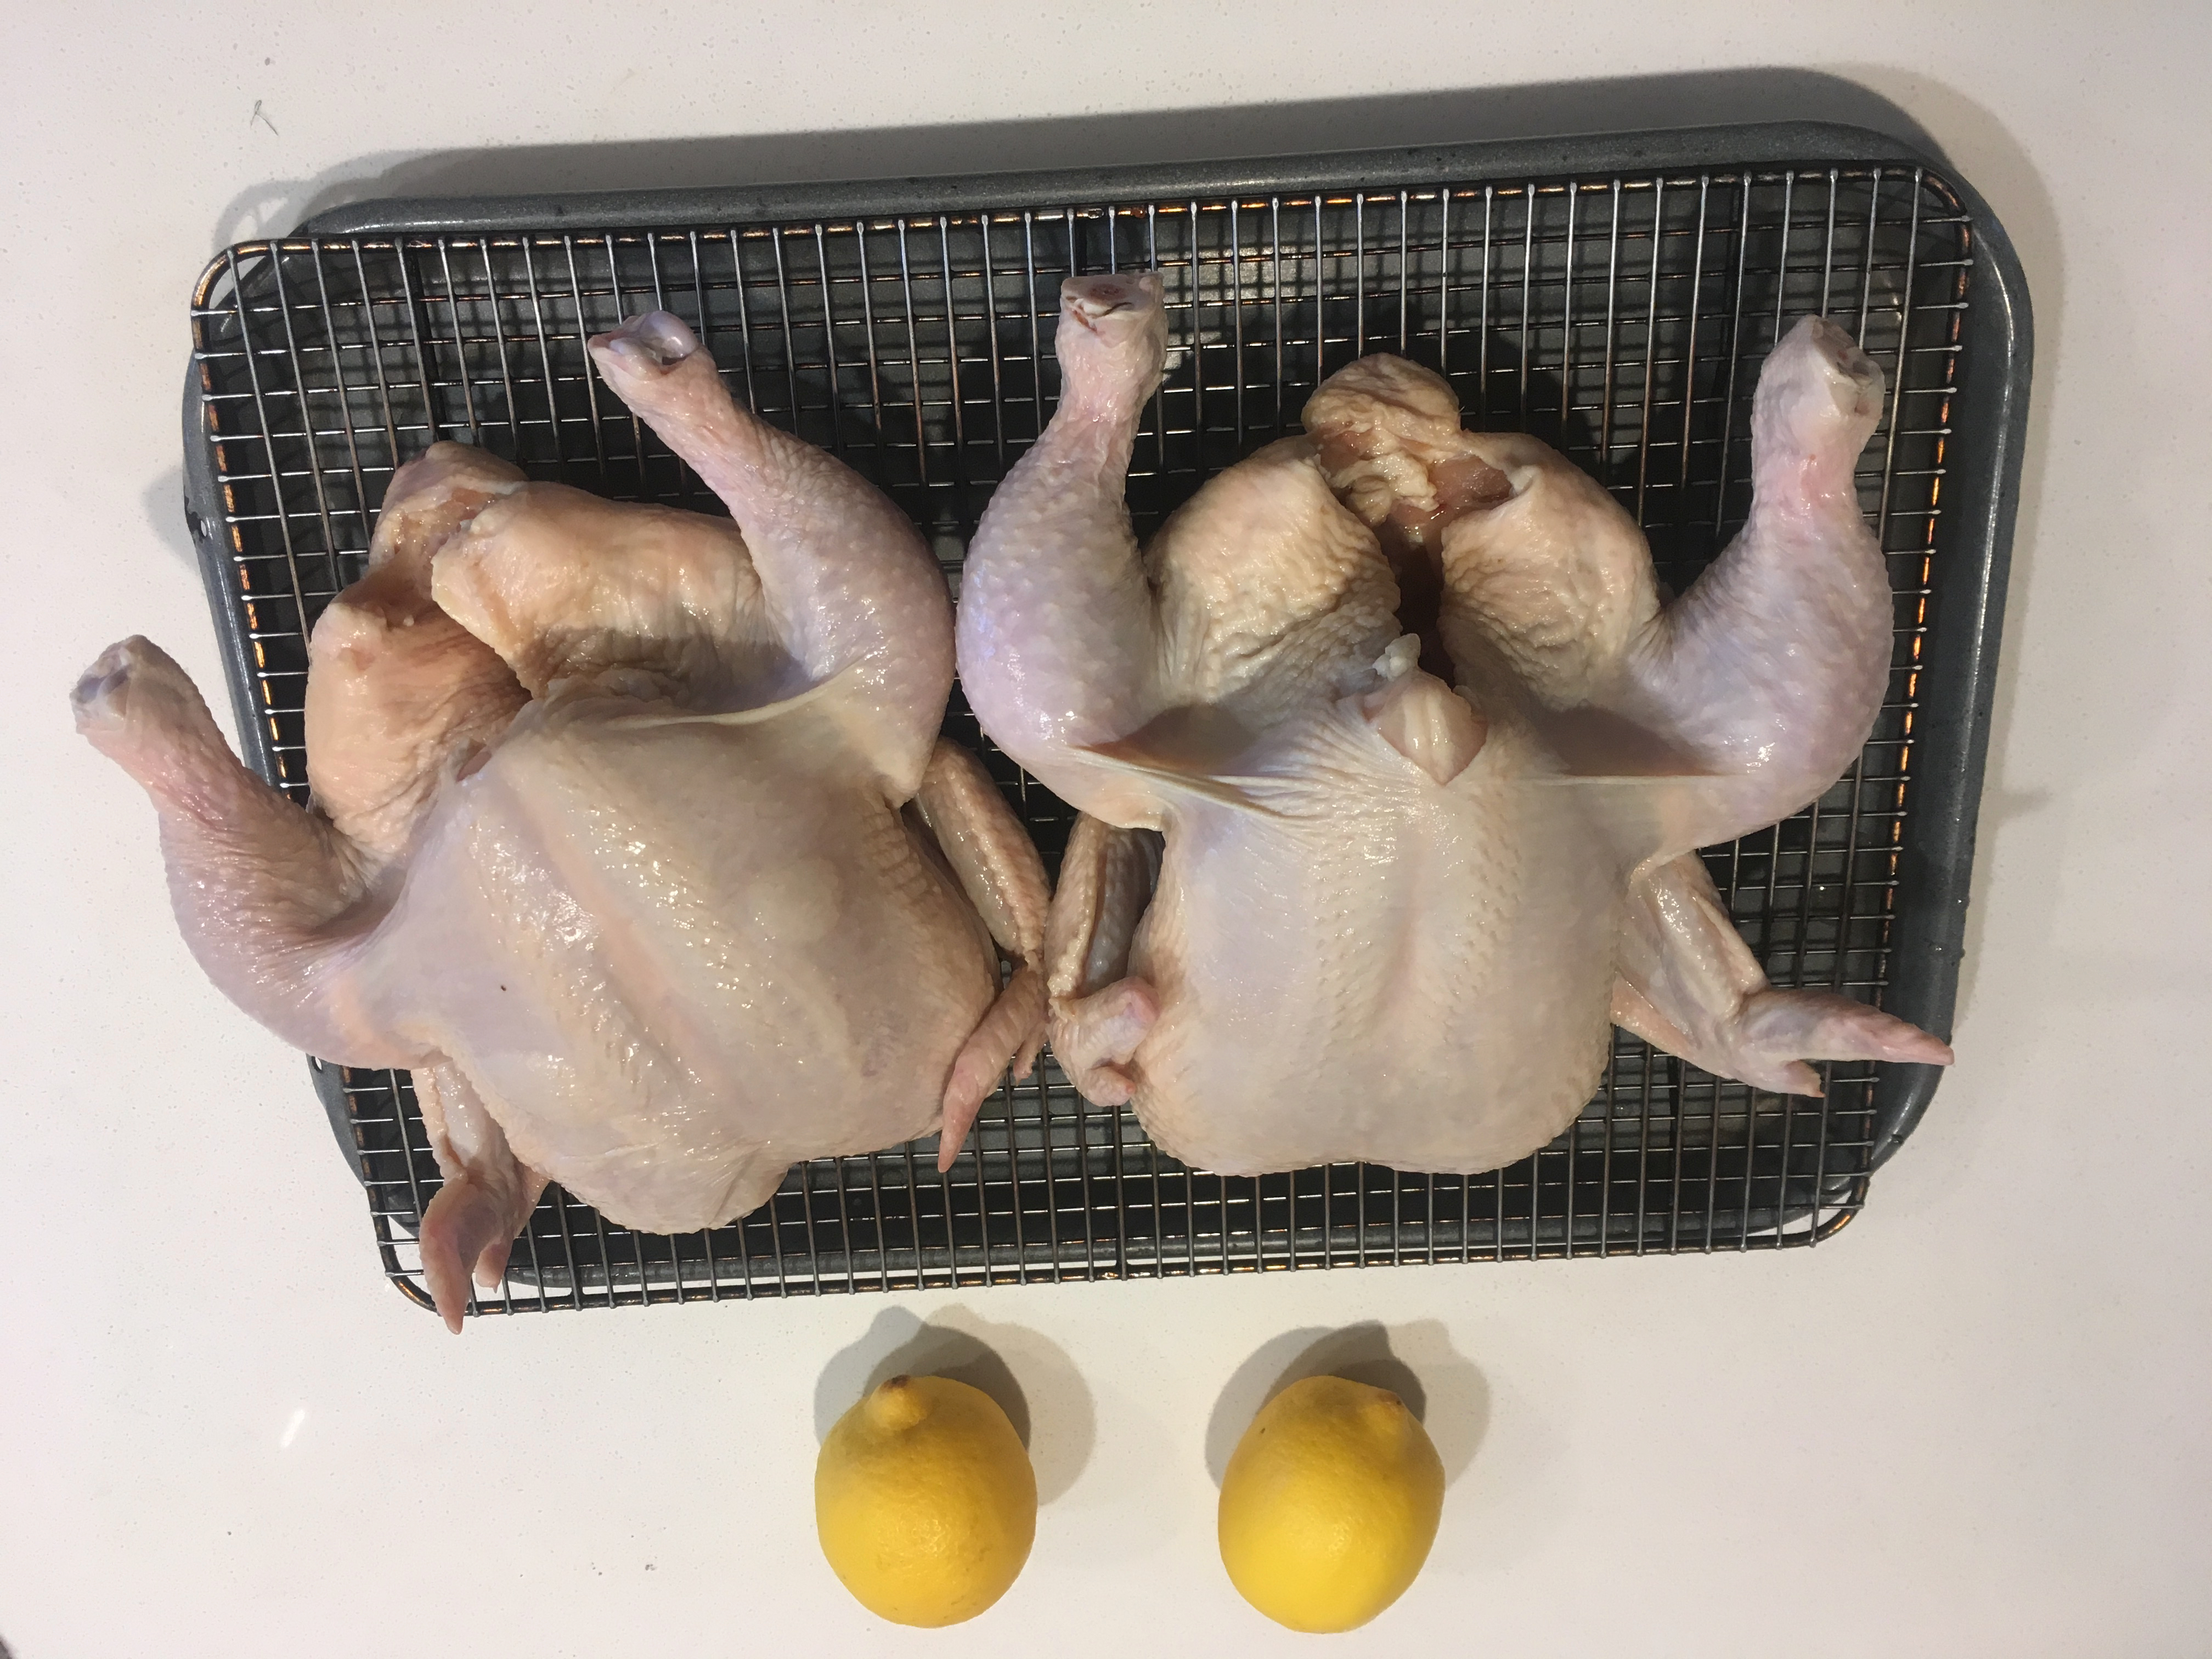
\includegraphics[width=0.25\textwidth]{\imageDir/\fileName/IMG_3197.jpg} &
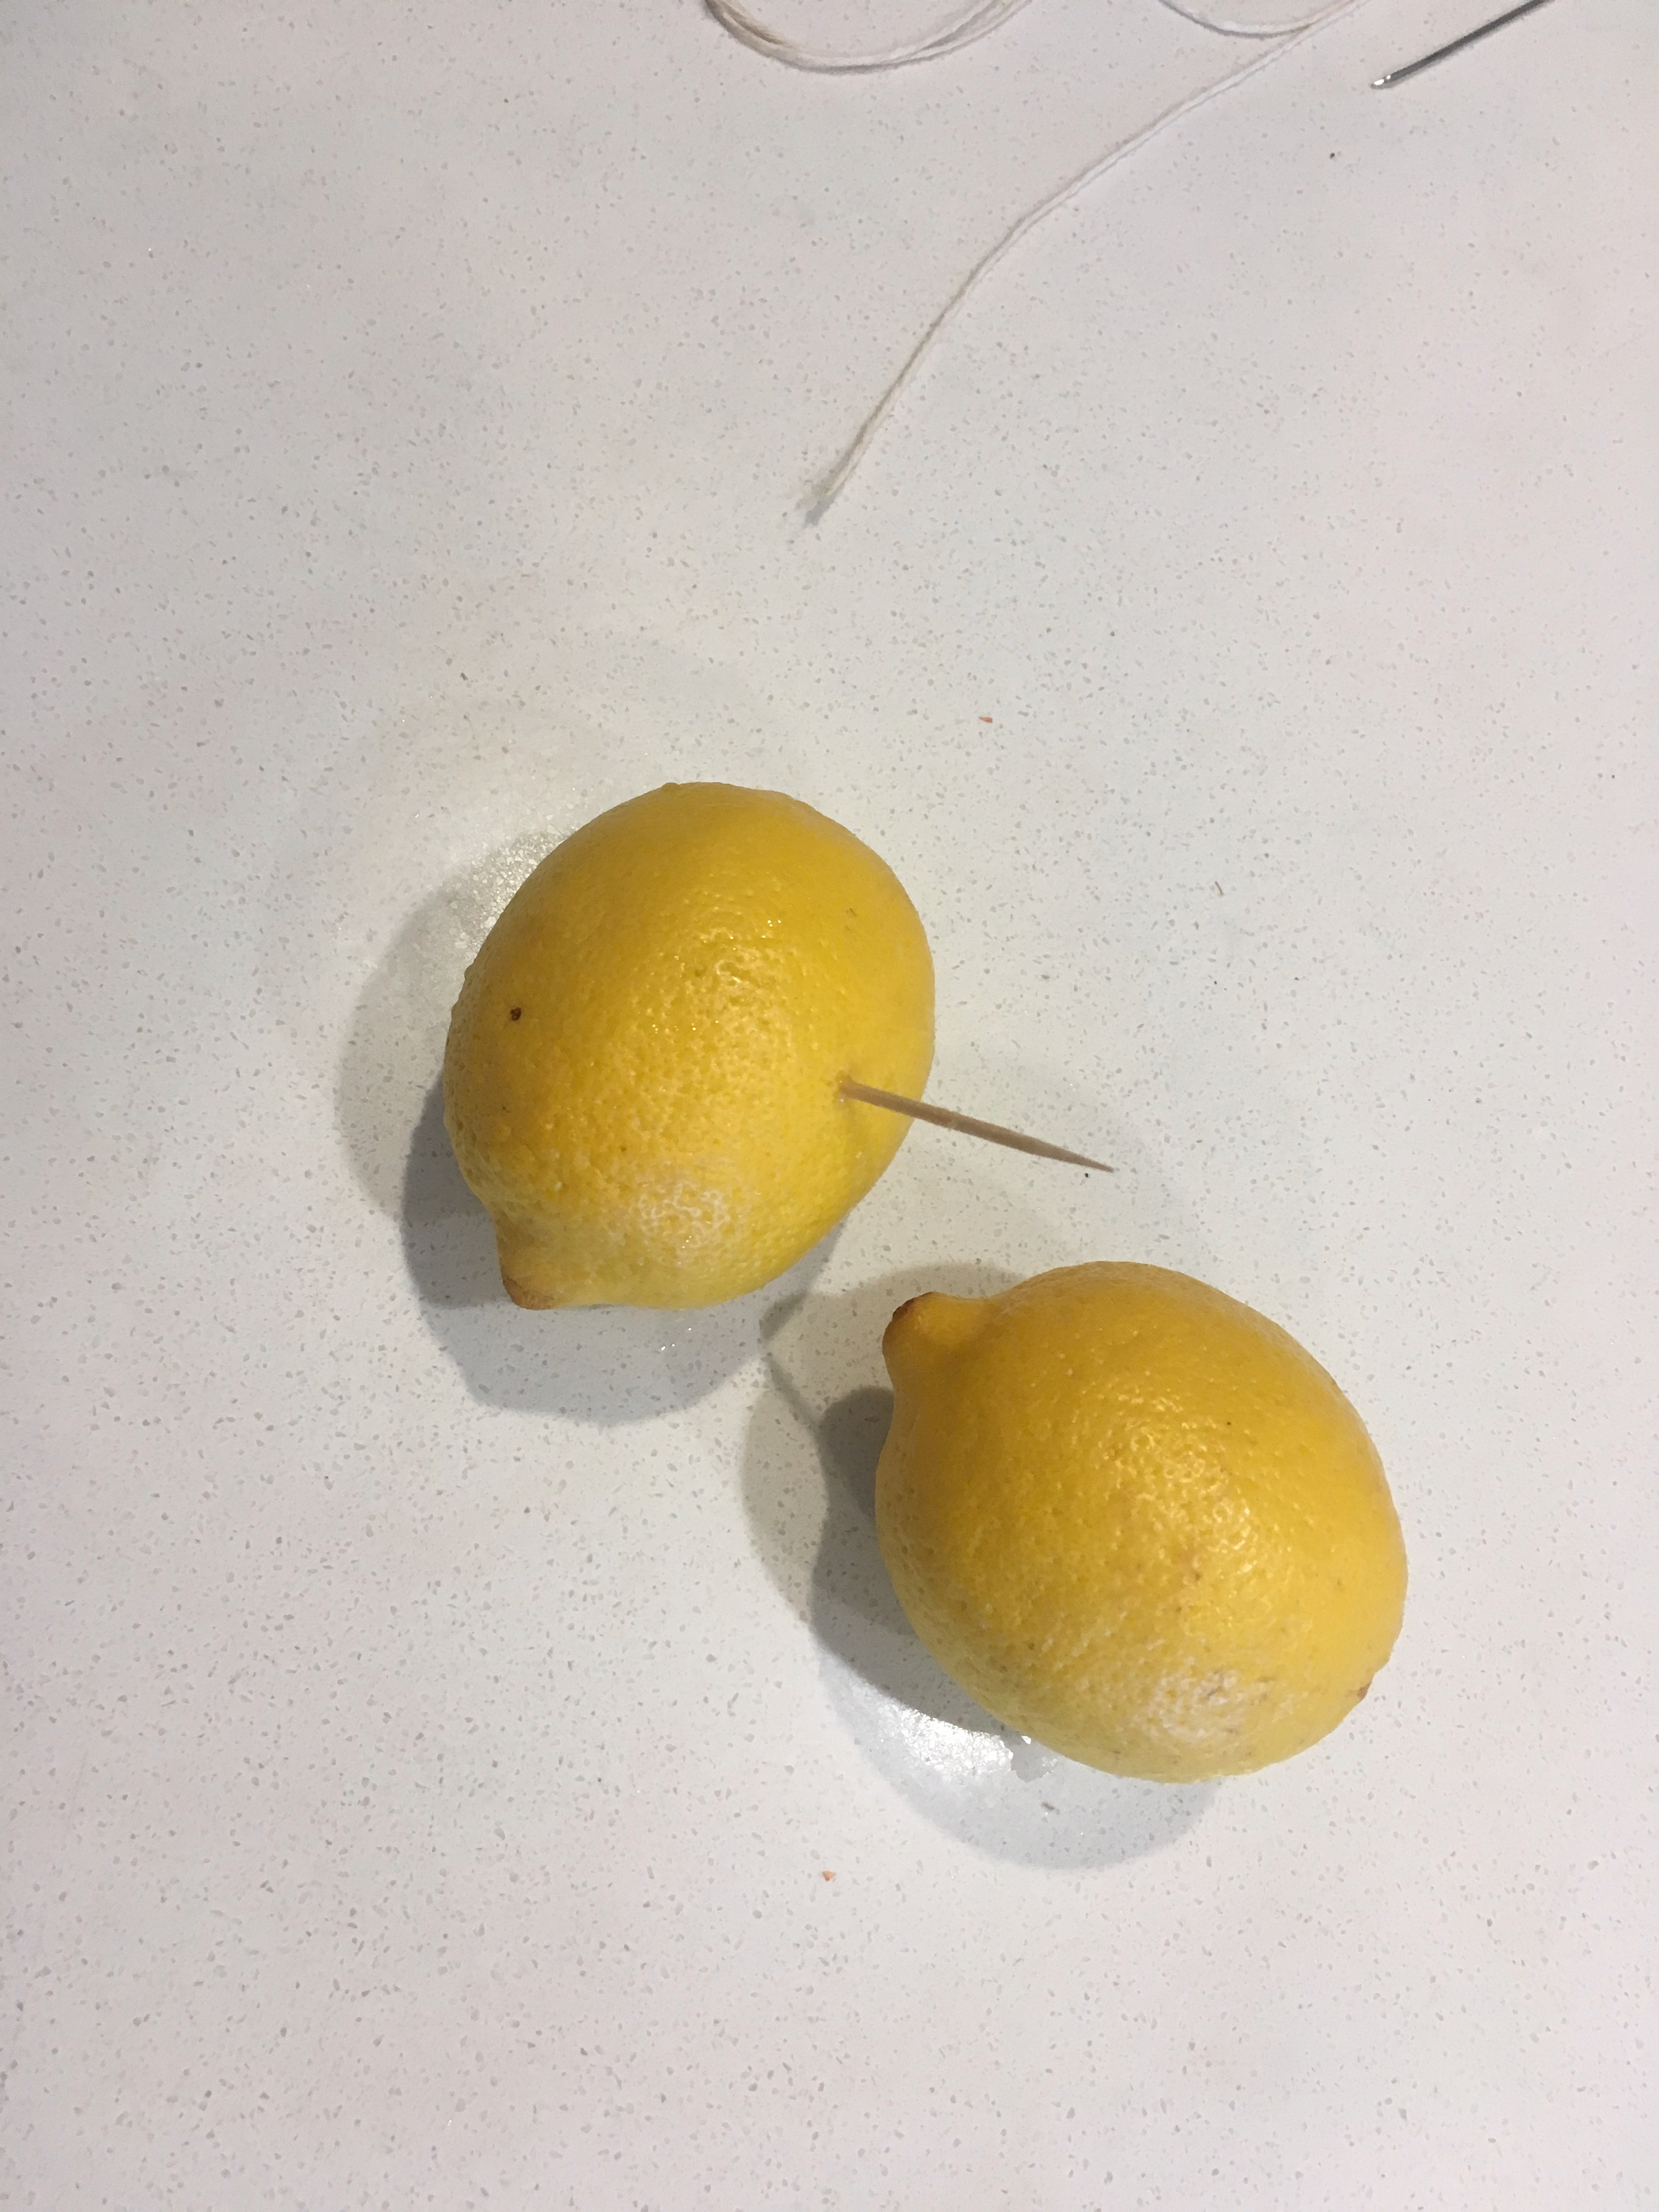
\includegraphics[width=0.25\textwidth]{\imageDir/\fileName/IMG_3212.jpg} &
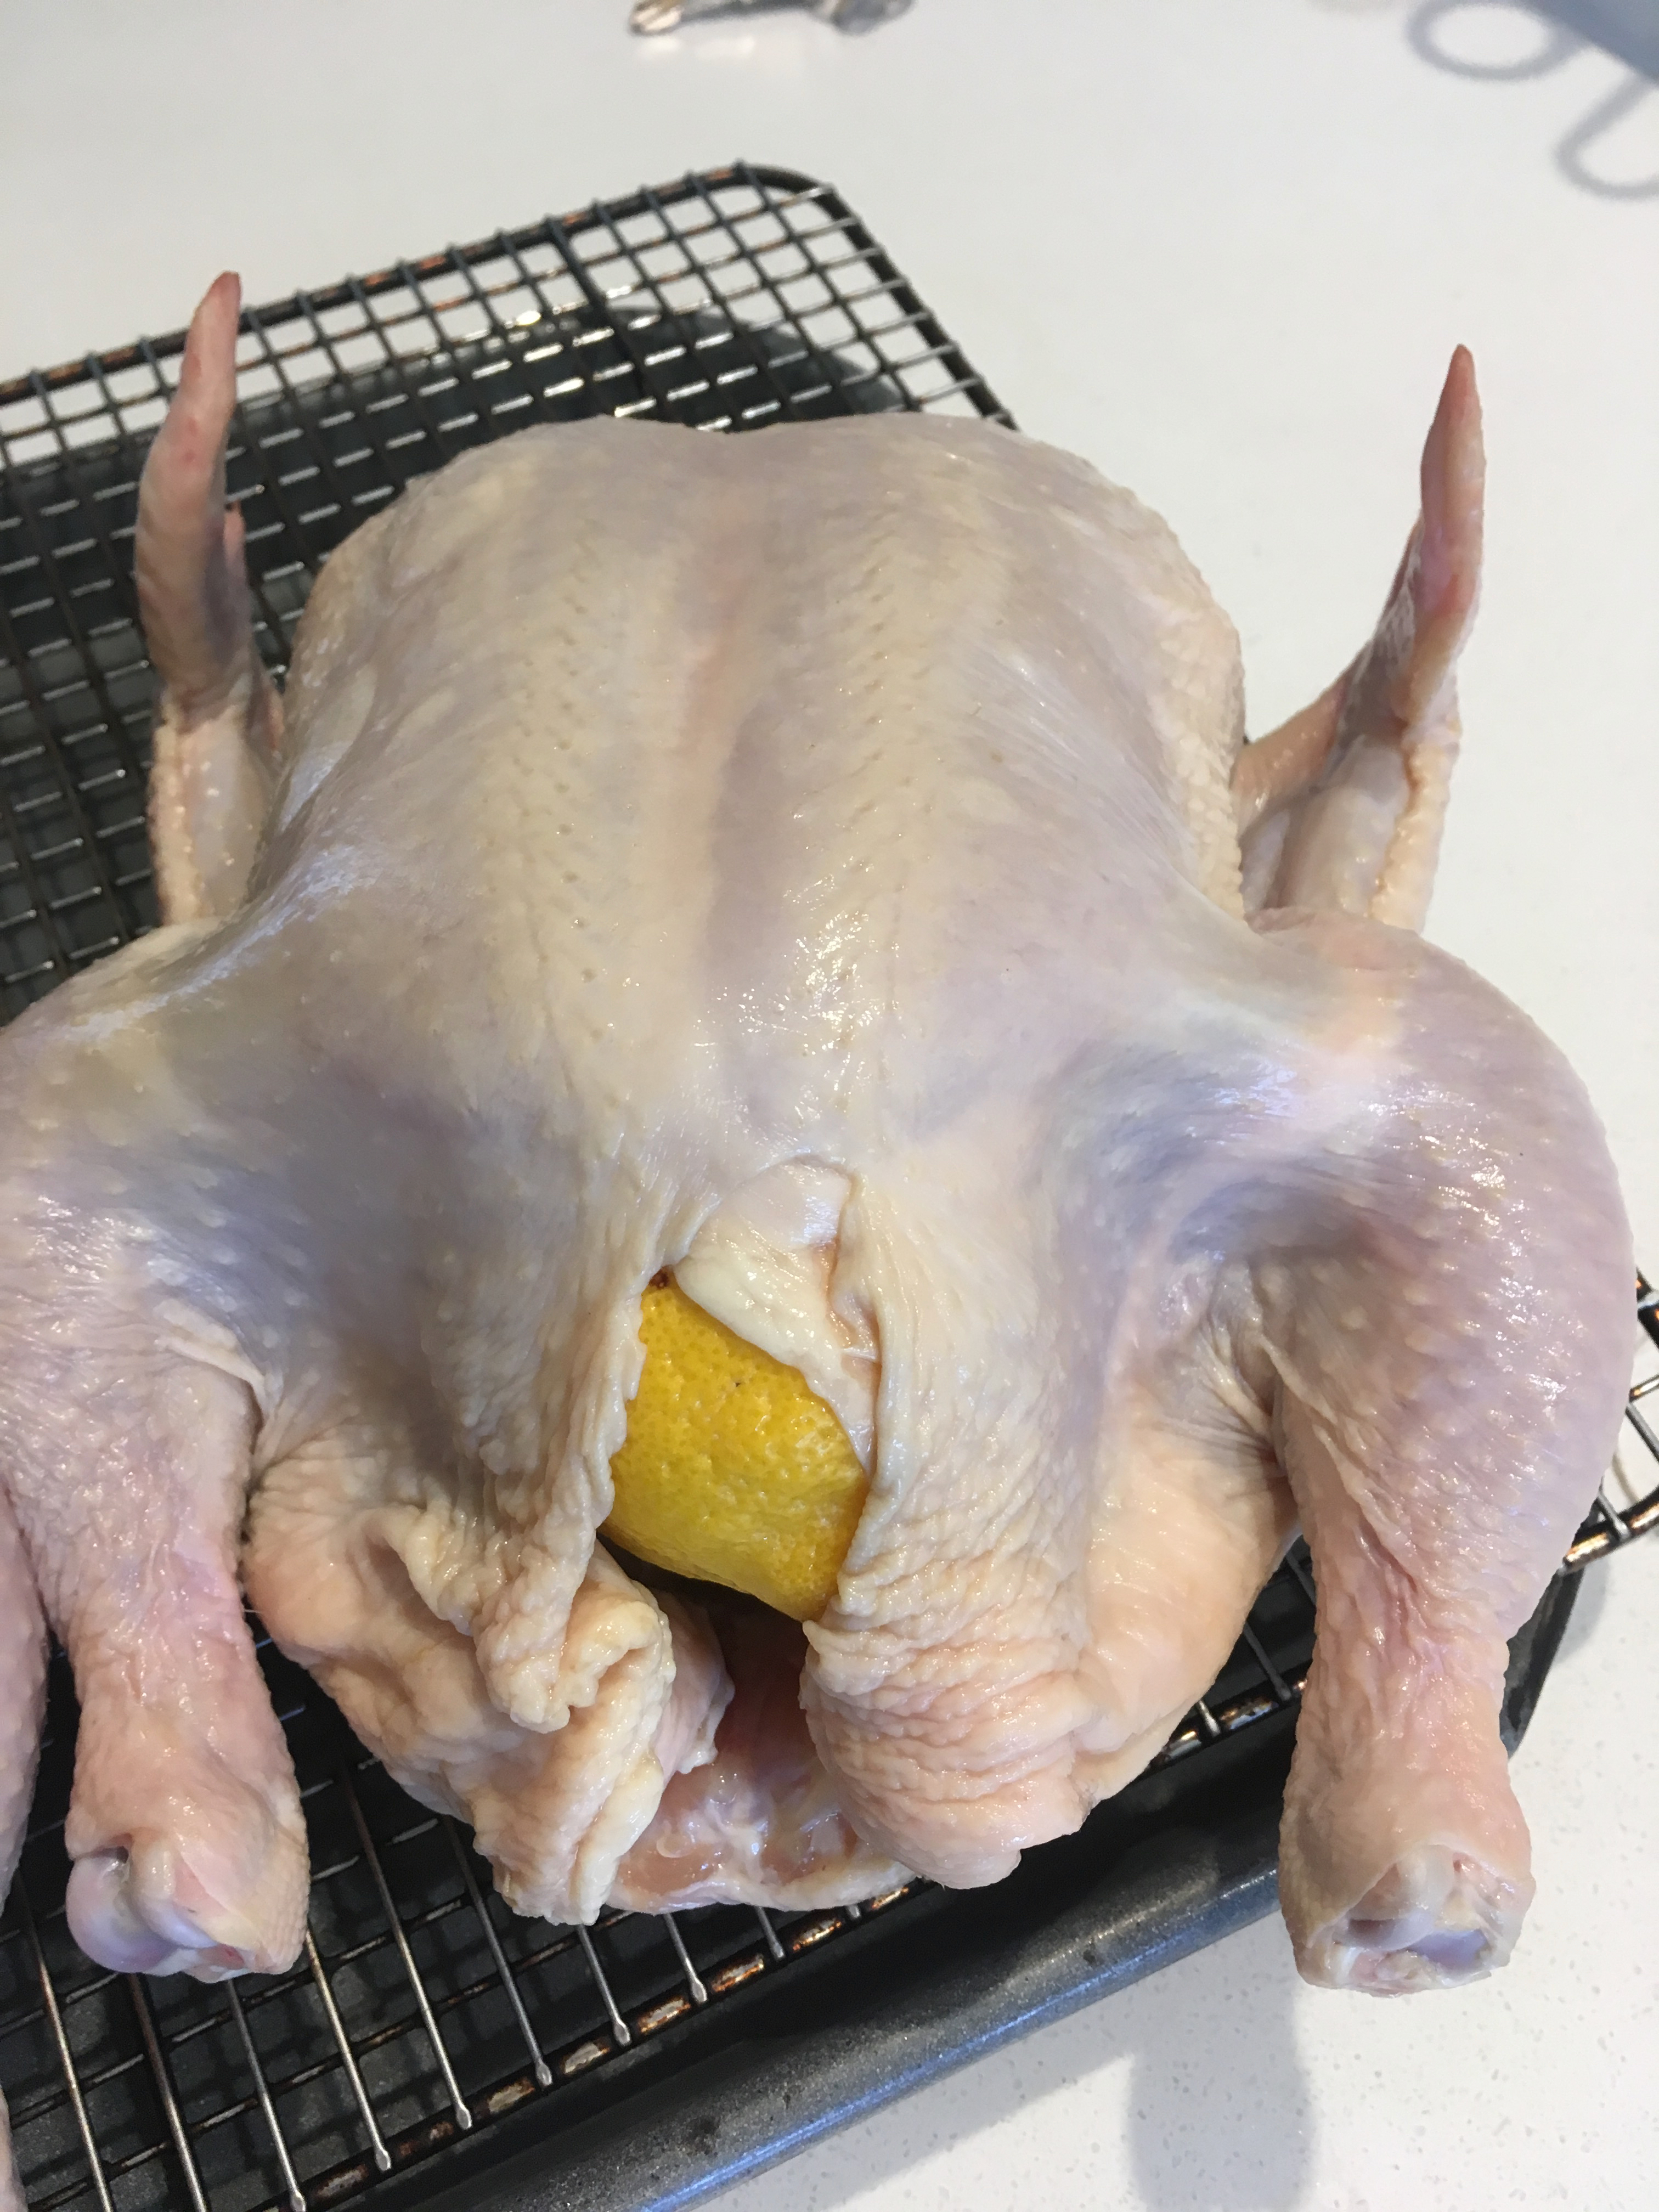
\includegraphics[width=0.25\textwidth]{\imageDir/\fileName/IMG_3213.jpg} \\
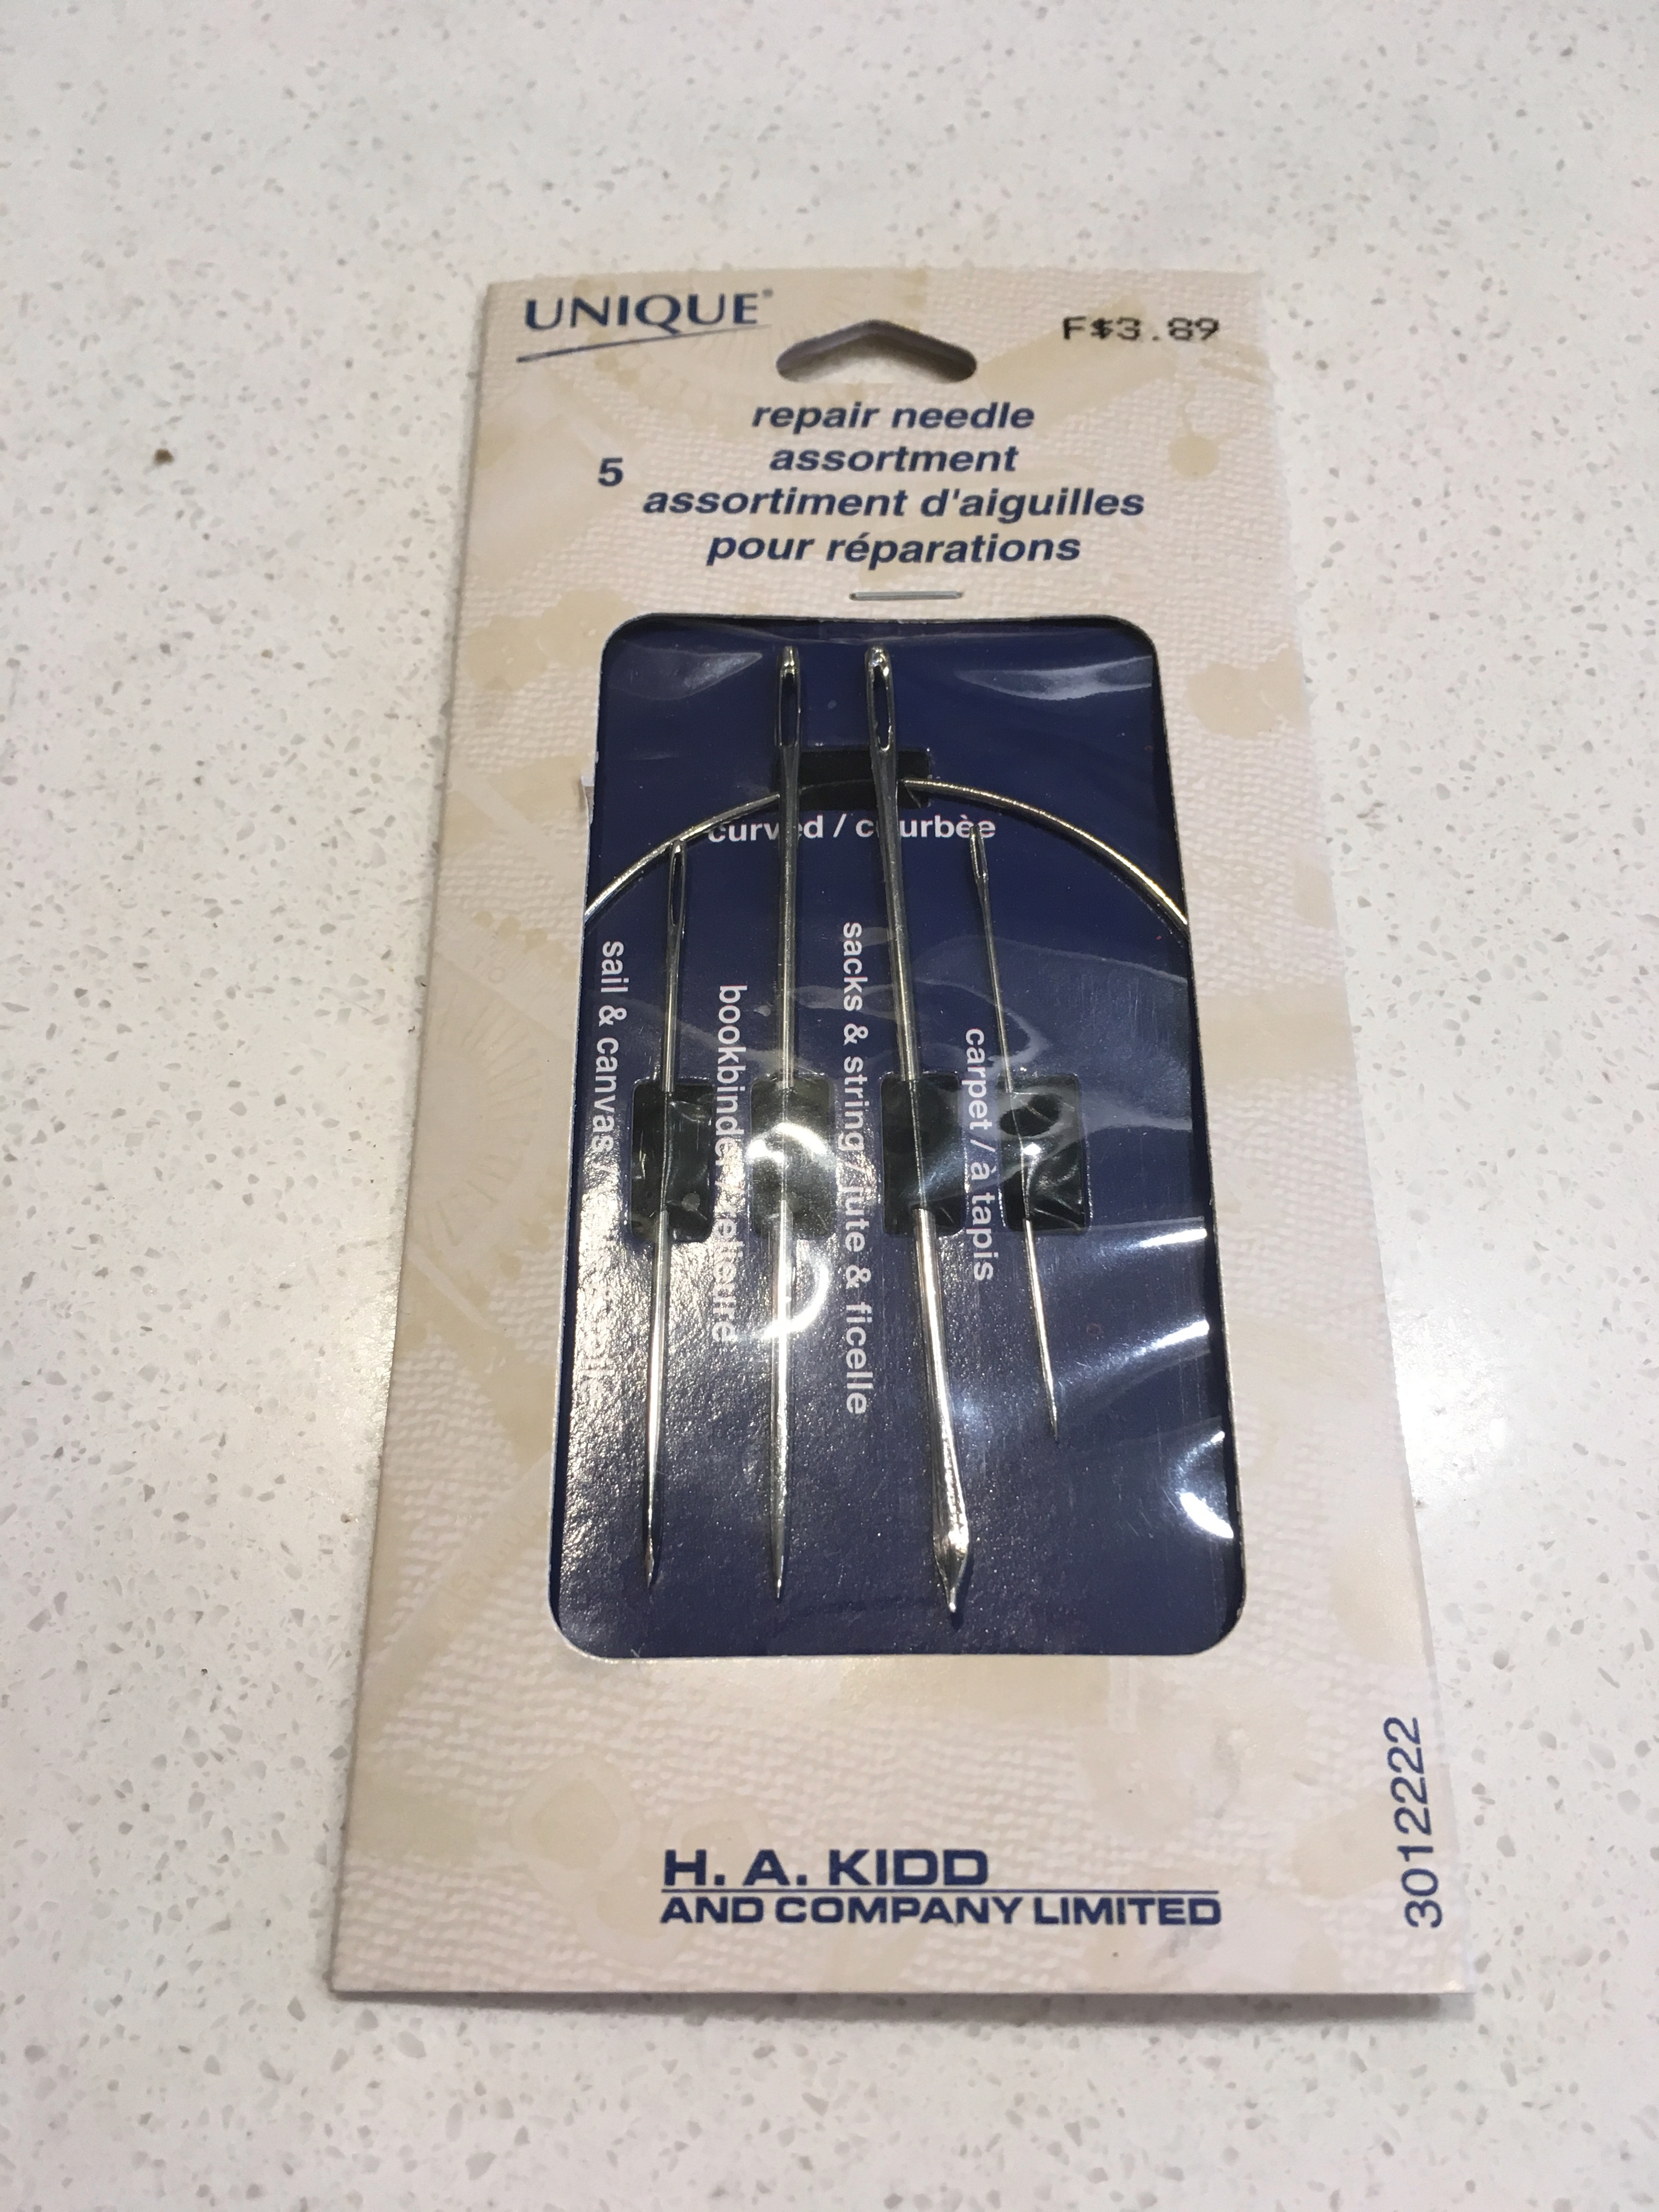
\includegraphics[width=0.25\textwidth]{\imageDir/\fileName/IMG_3206.jpg} &
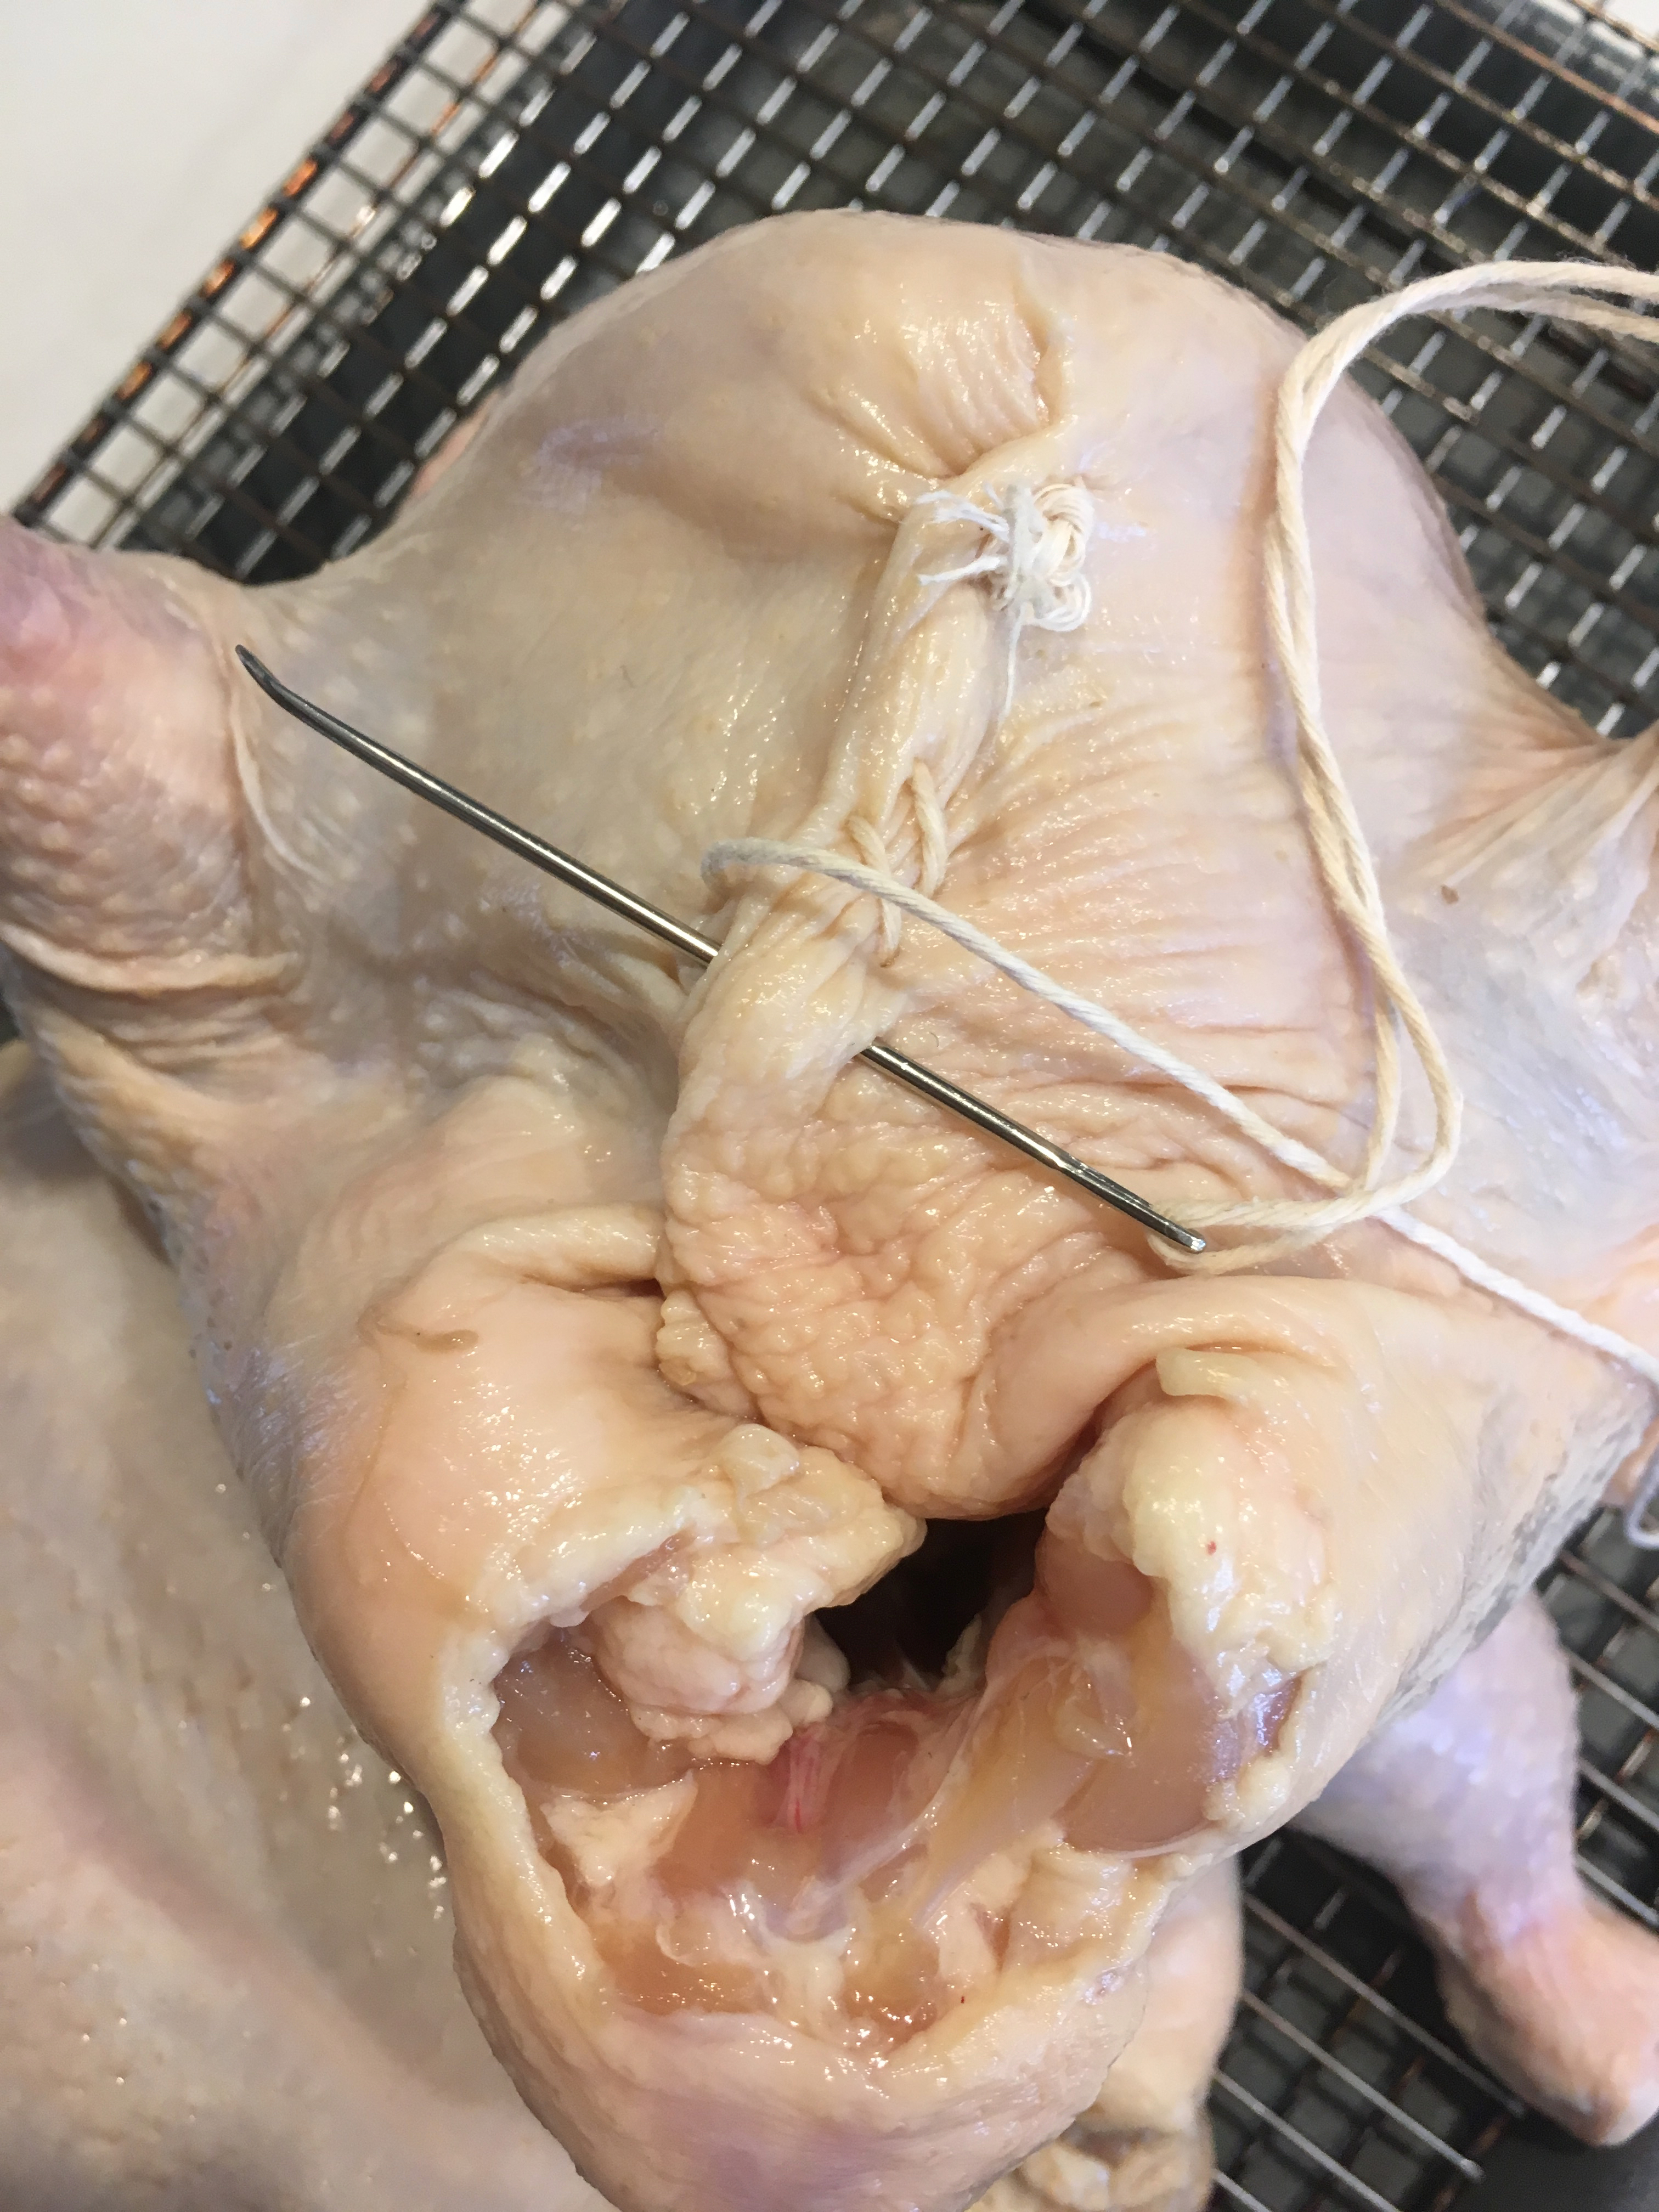
\includegraphics[width=0.25\textwidth]{\imageDir/\fileName/IMG_3214.jpg} &
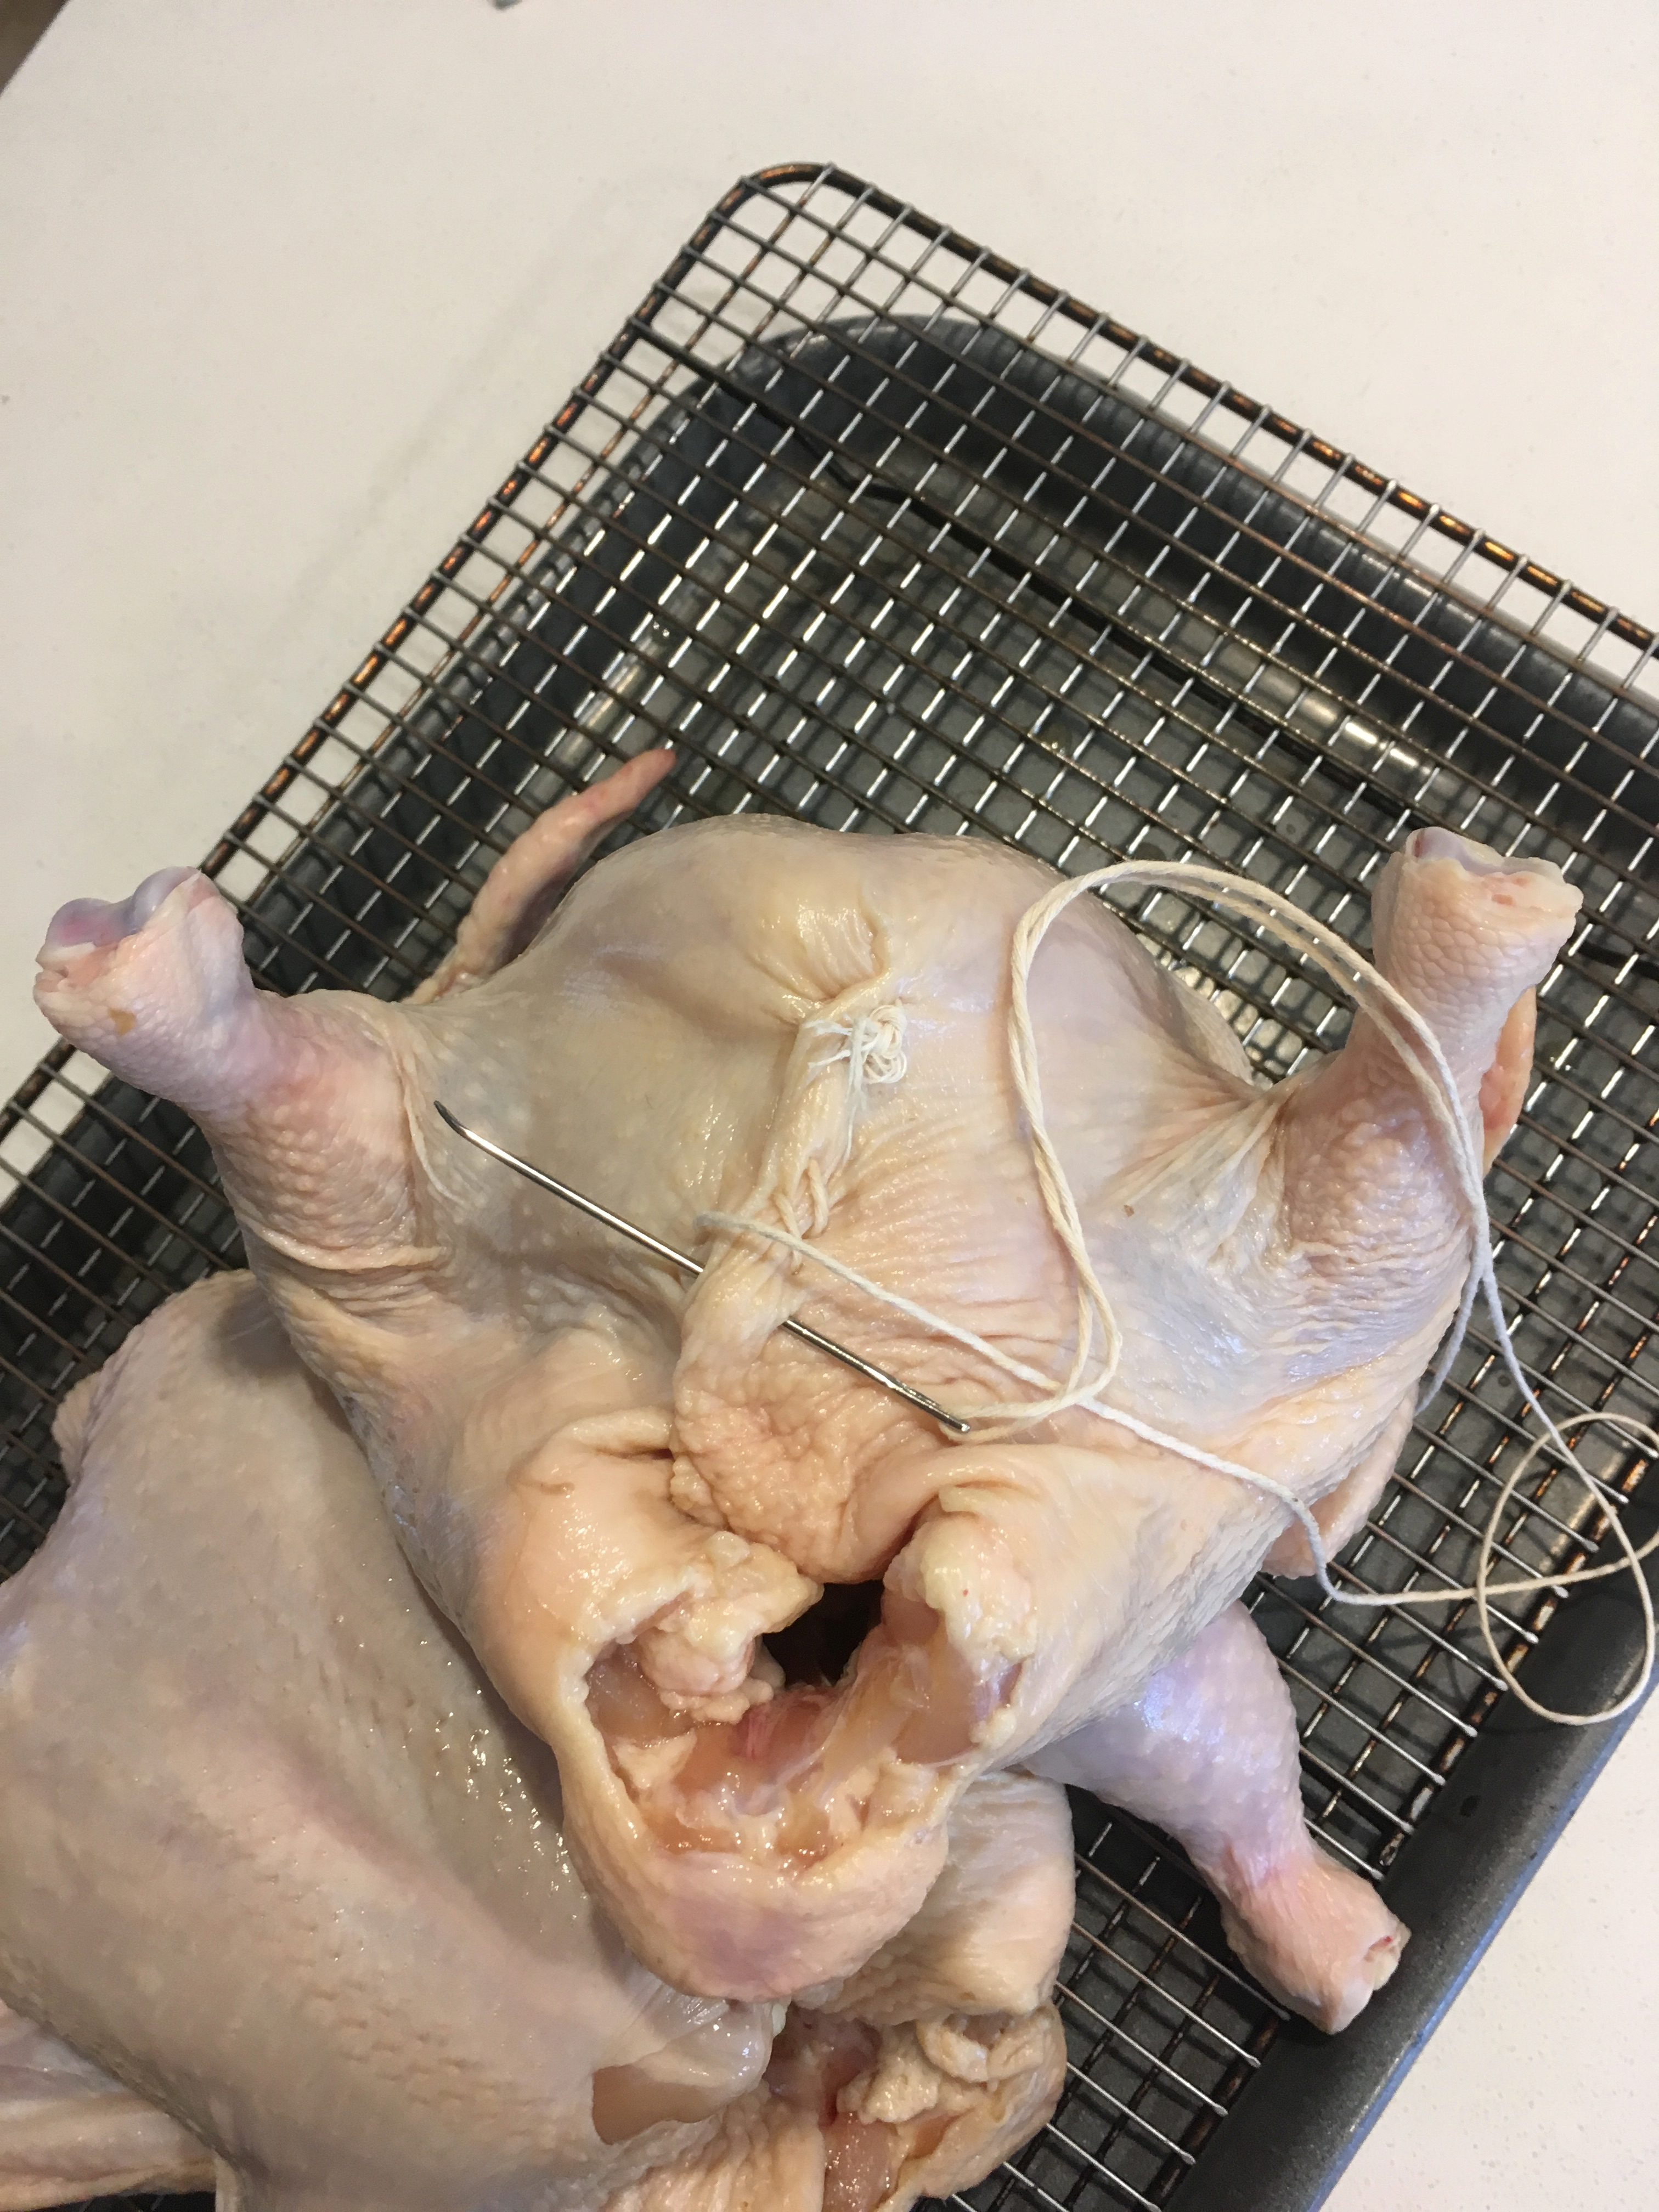
\includegraphics[width=0.25\textwidth]{\imageDir/\fileName/IMG_3216.jpg} \\
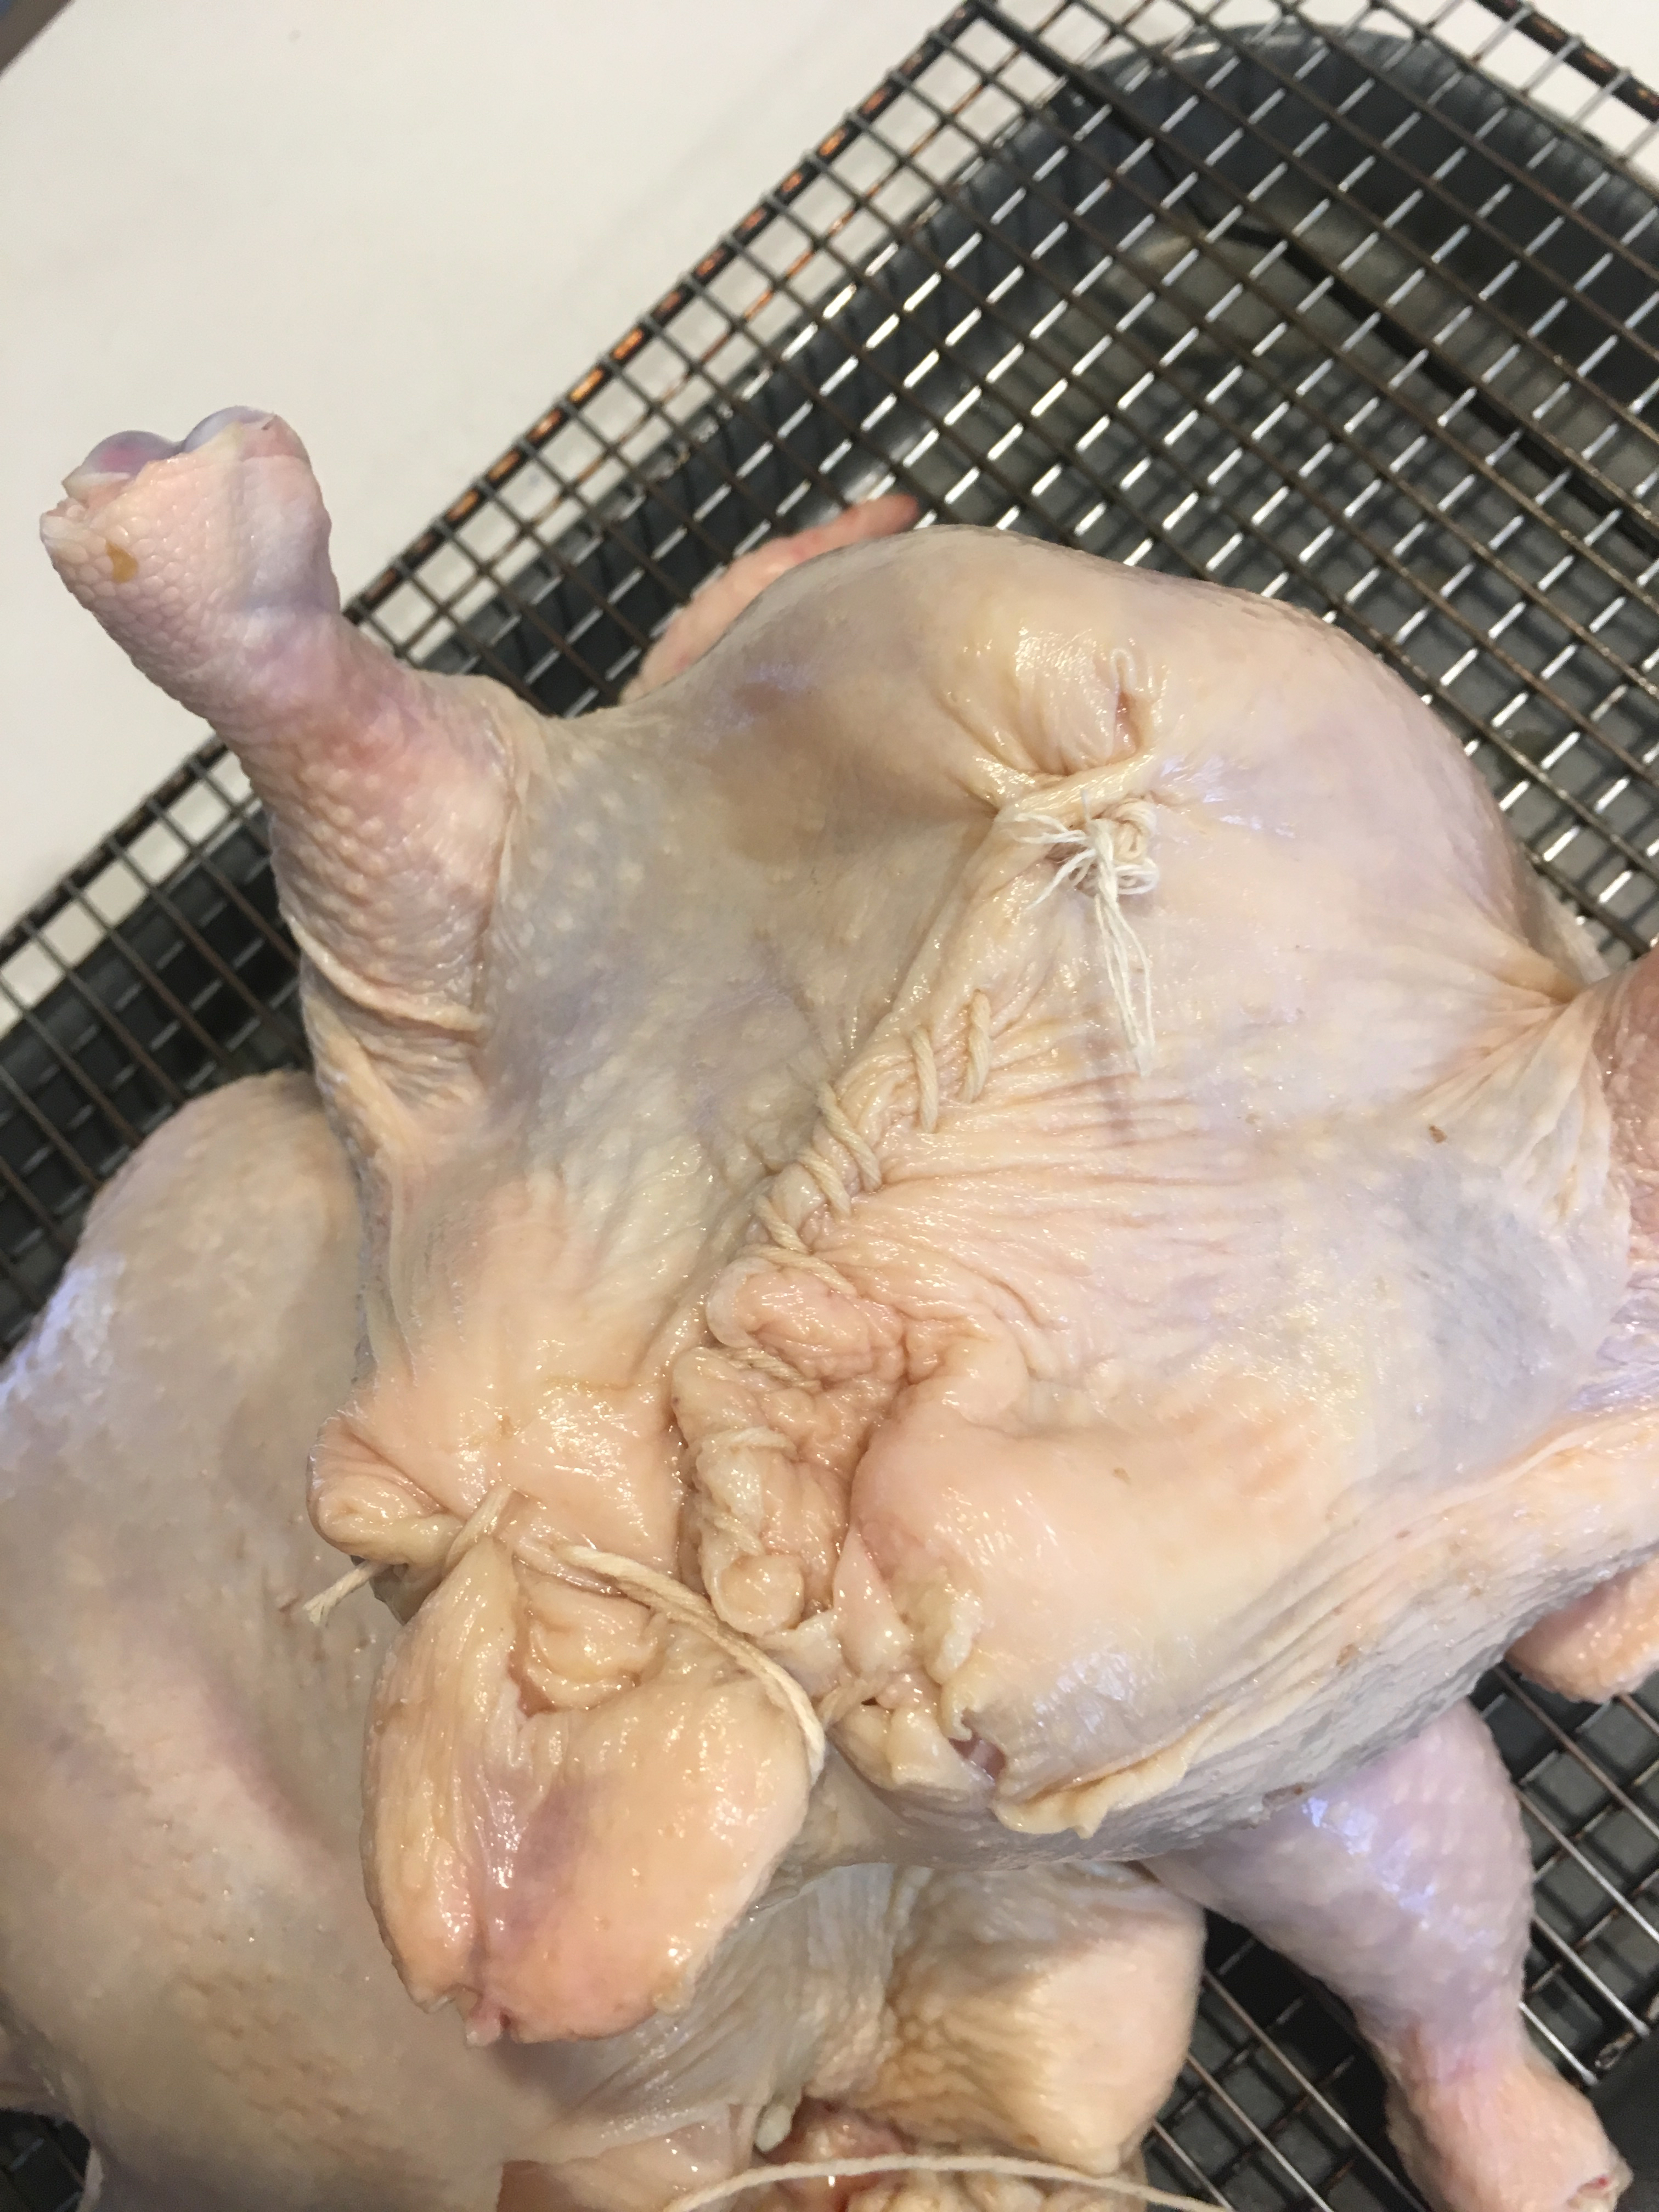
\includegraphics[width=0.25\textwidth]{\imageDir/\fileName/IMG_3217.jpg} &
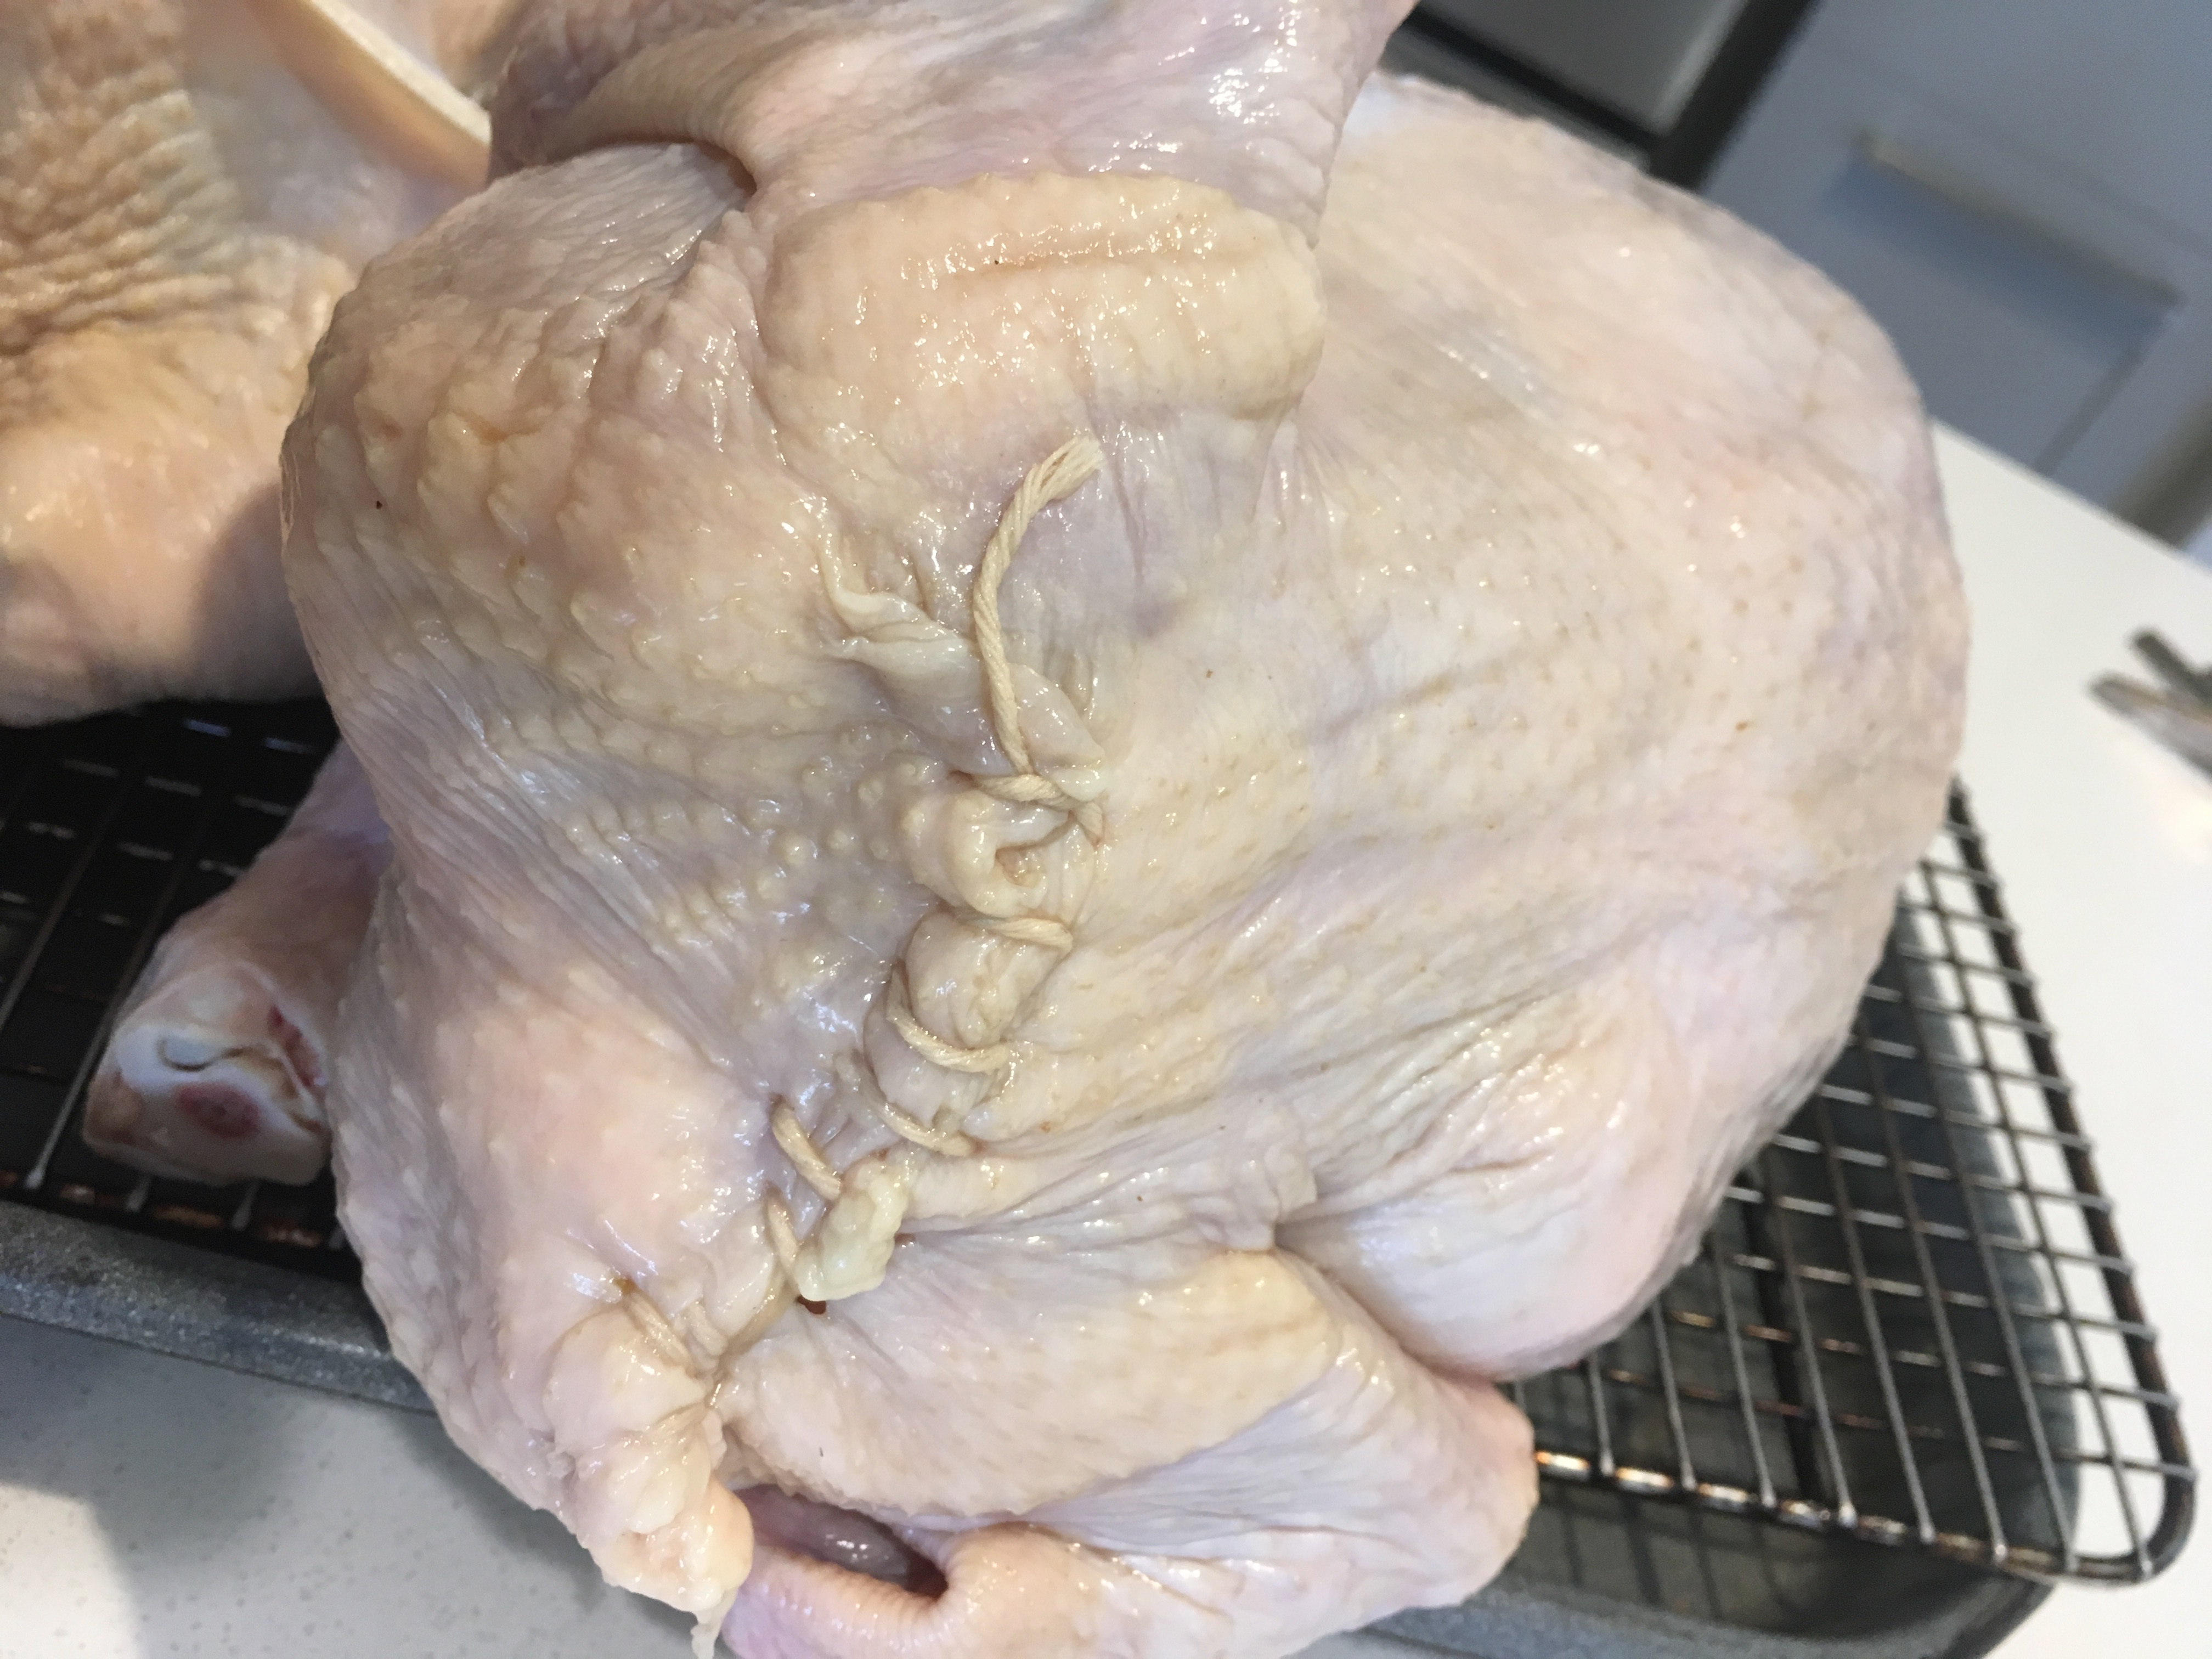
\includegraphics[width=0.25\textwidth]{\imageDir/\fileName/IMG_3218.jpg} &
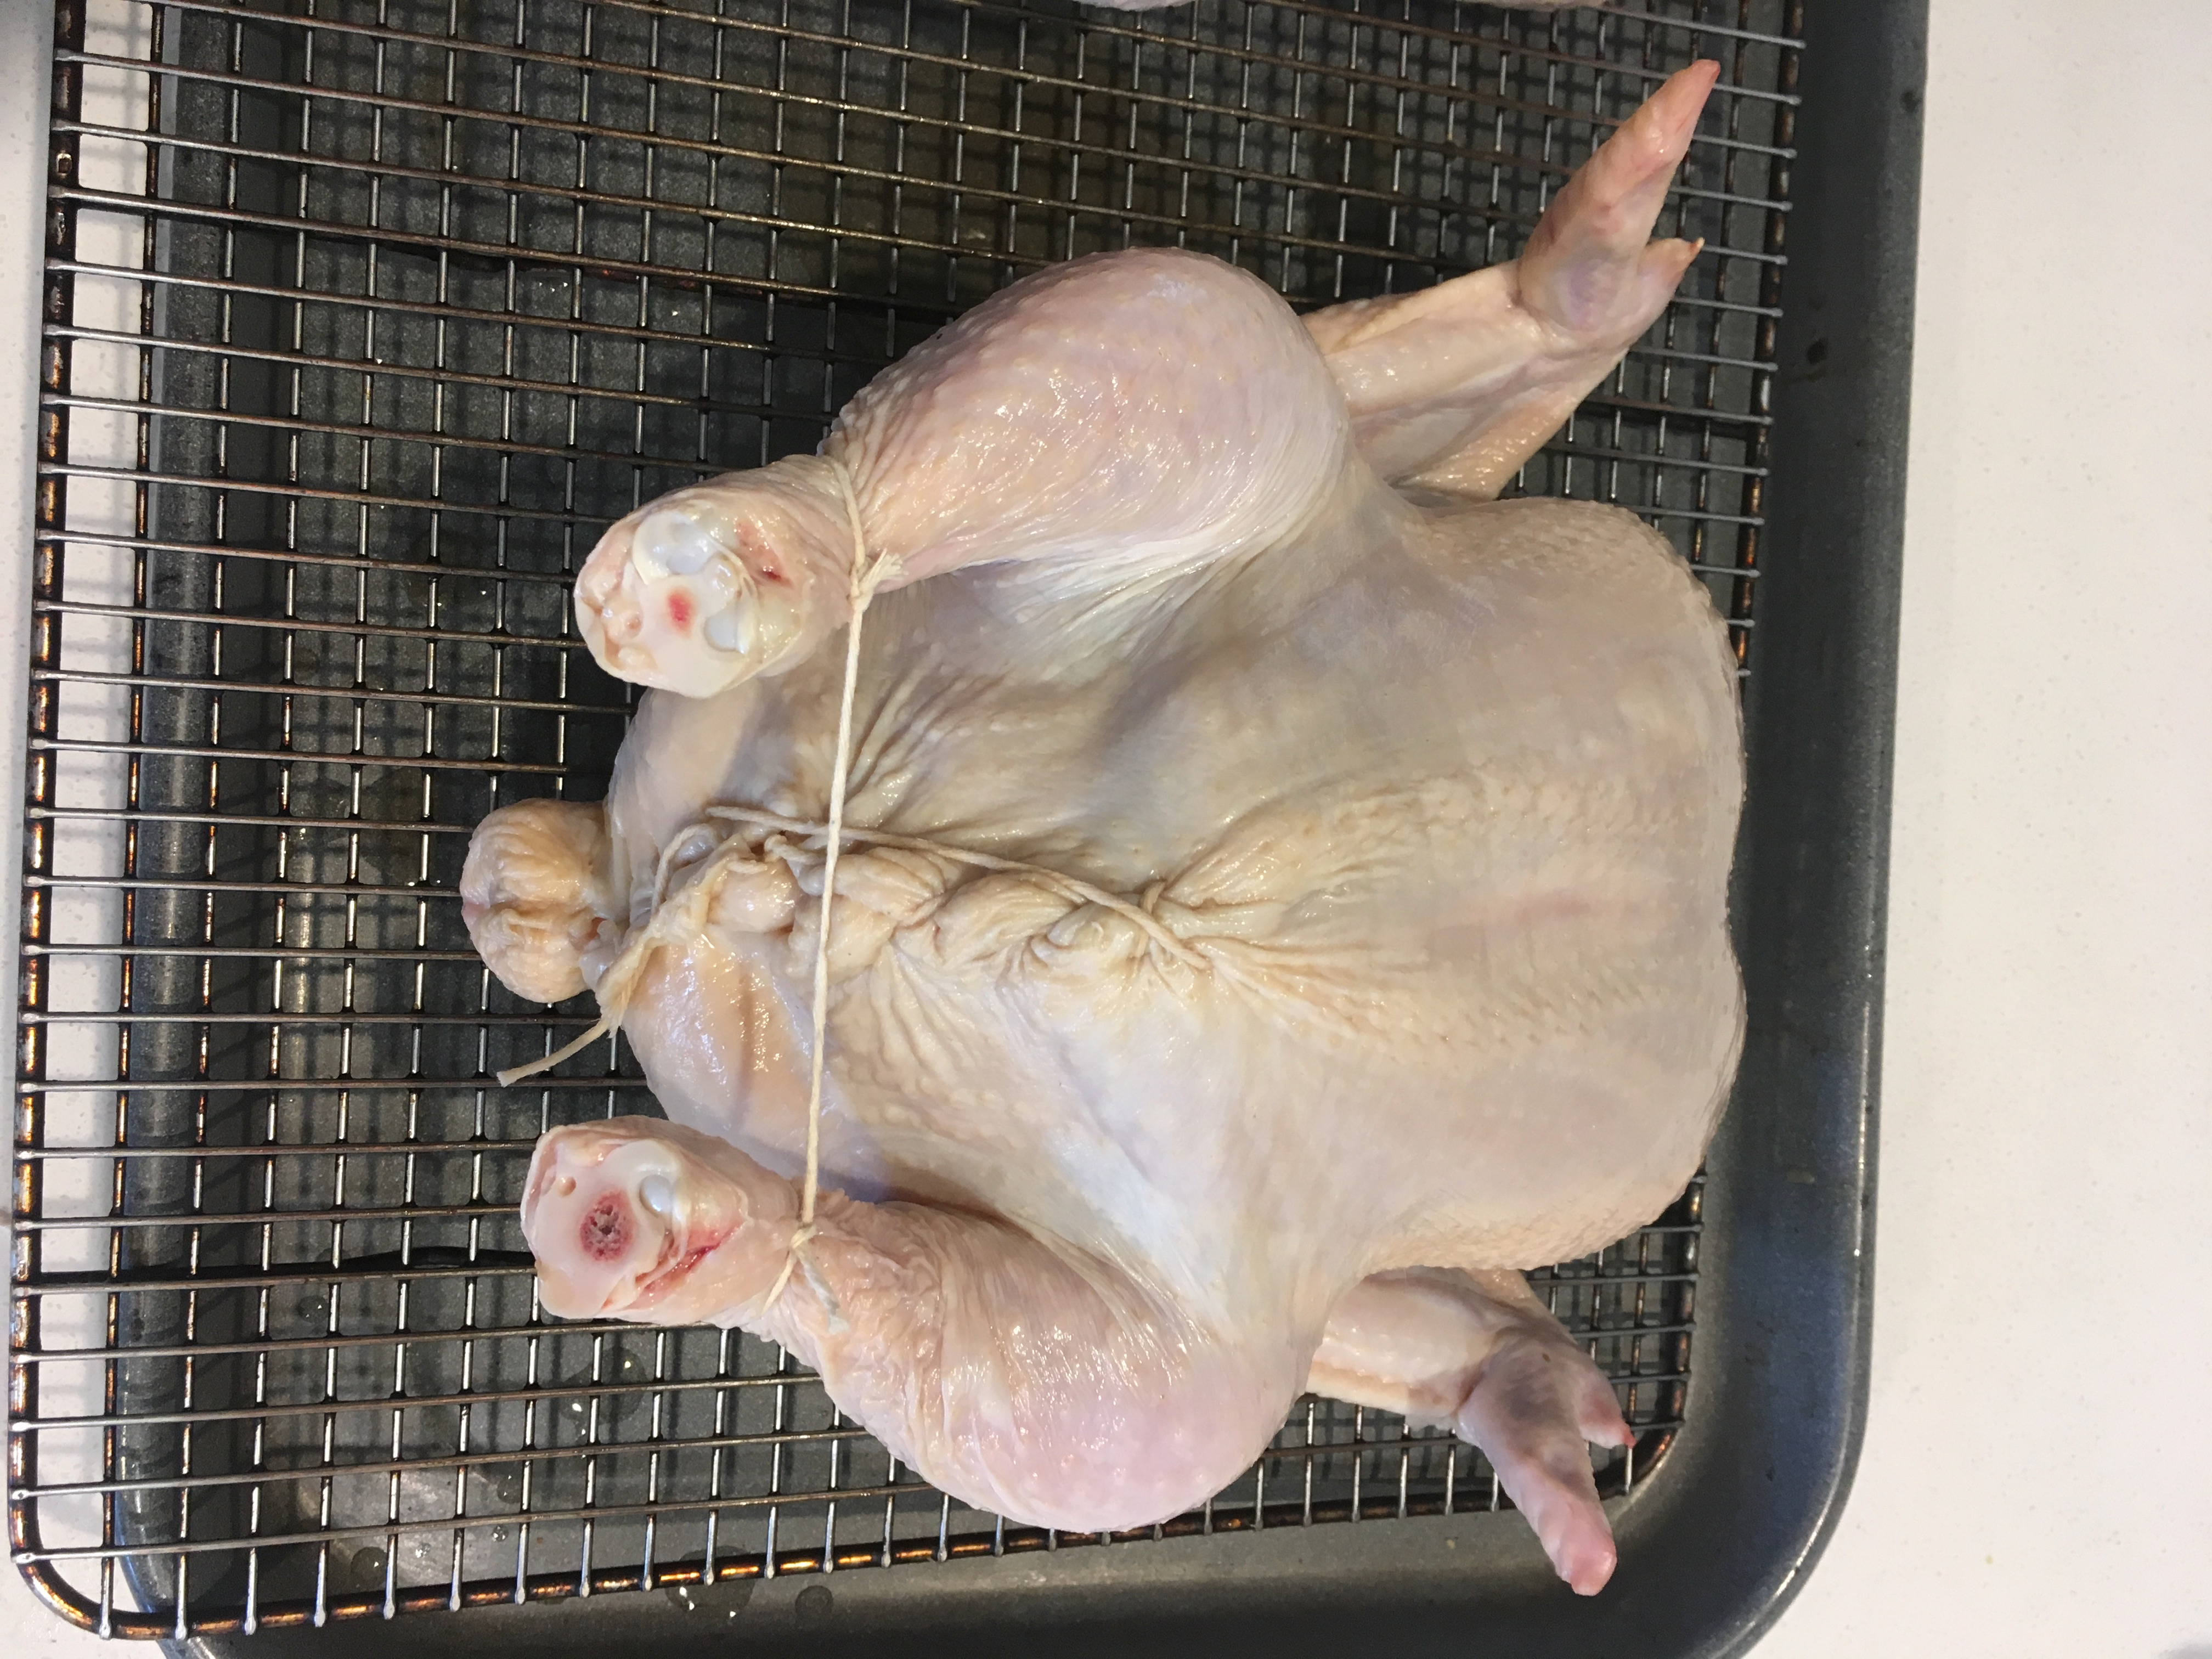
\includegraphics[width=0.25\textwidth]{\imageDir/\fileName/IMG_3219.jpg} \\
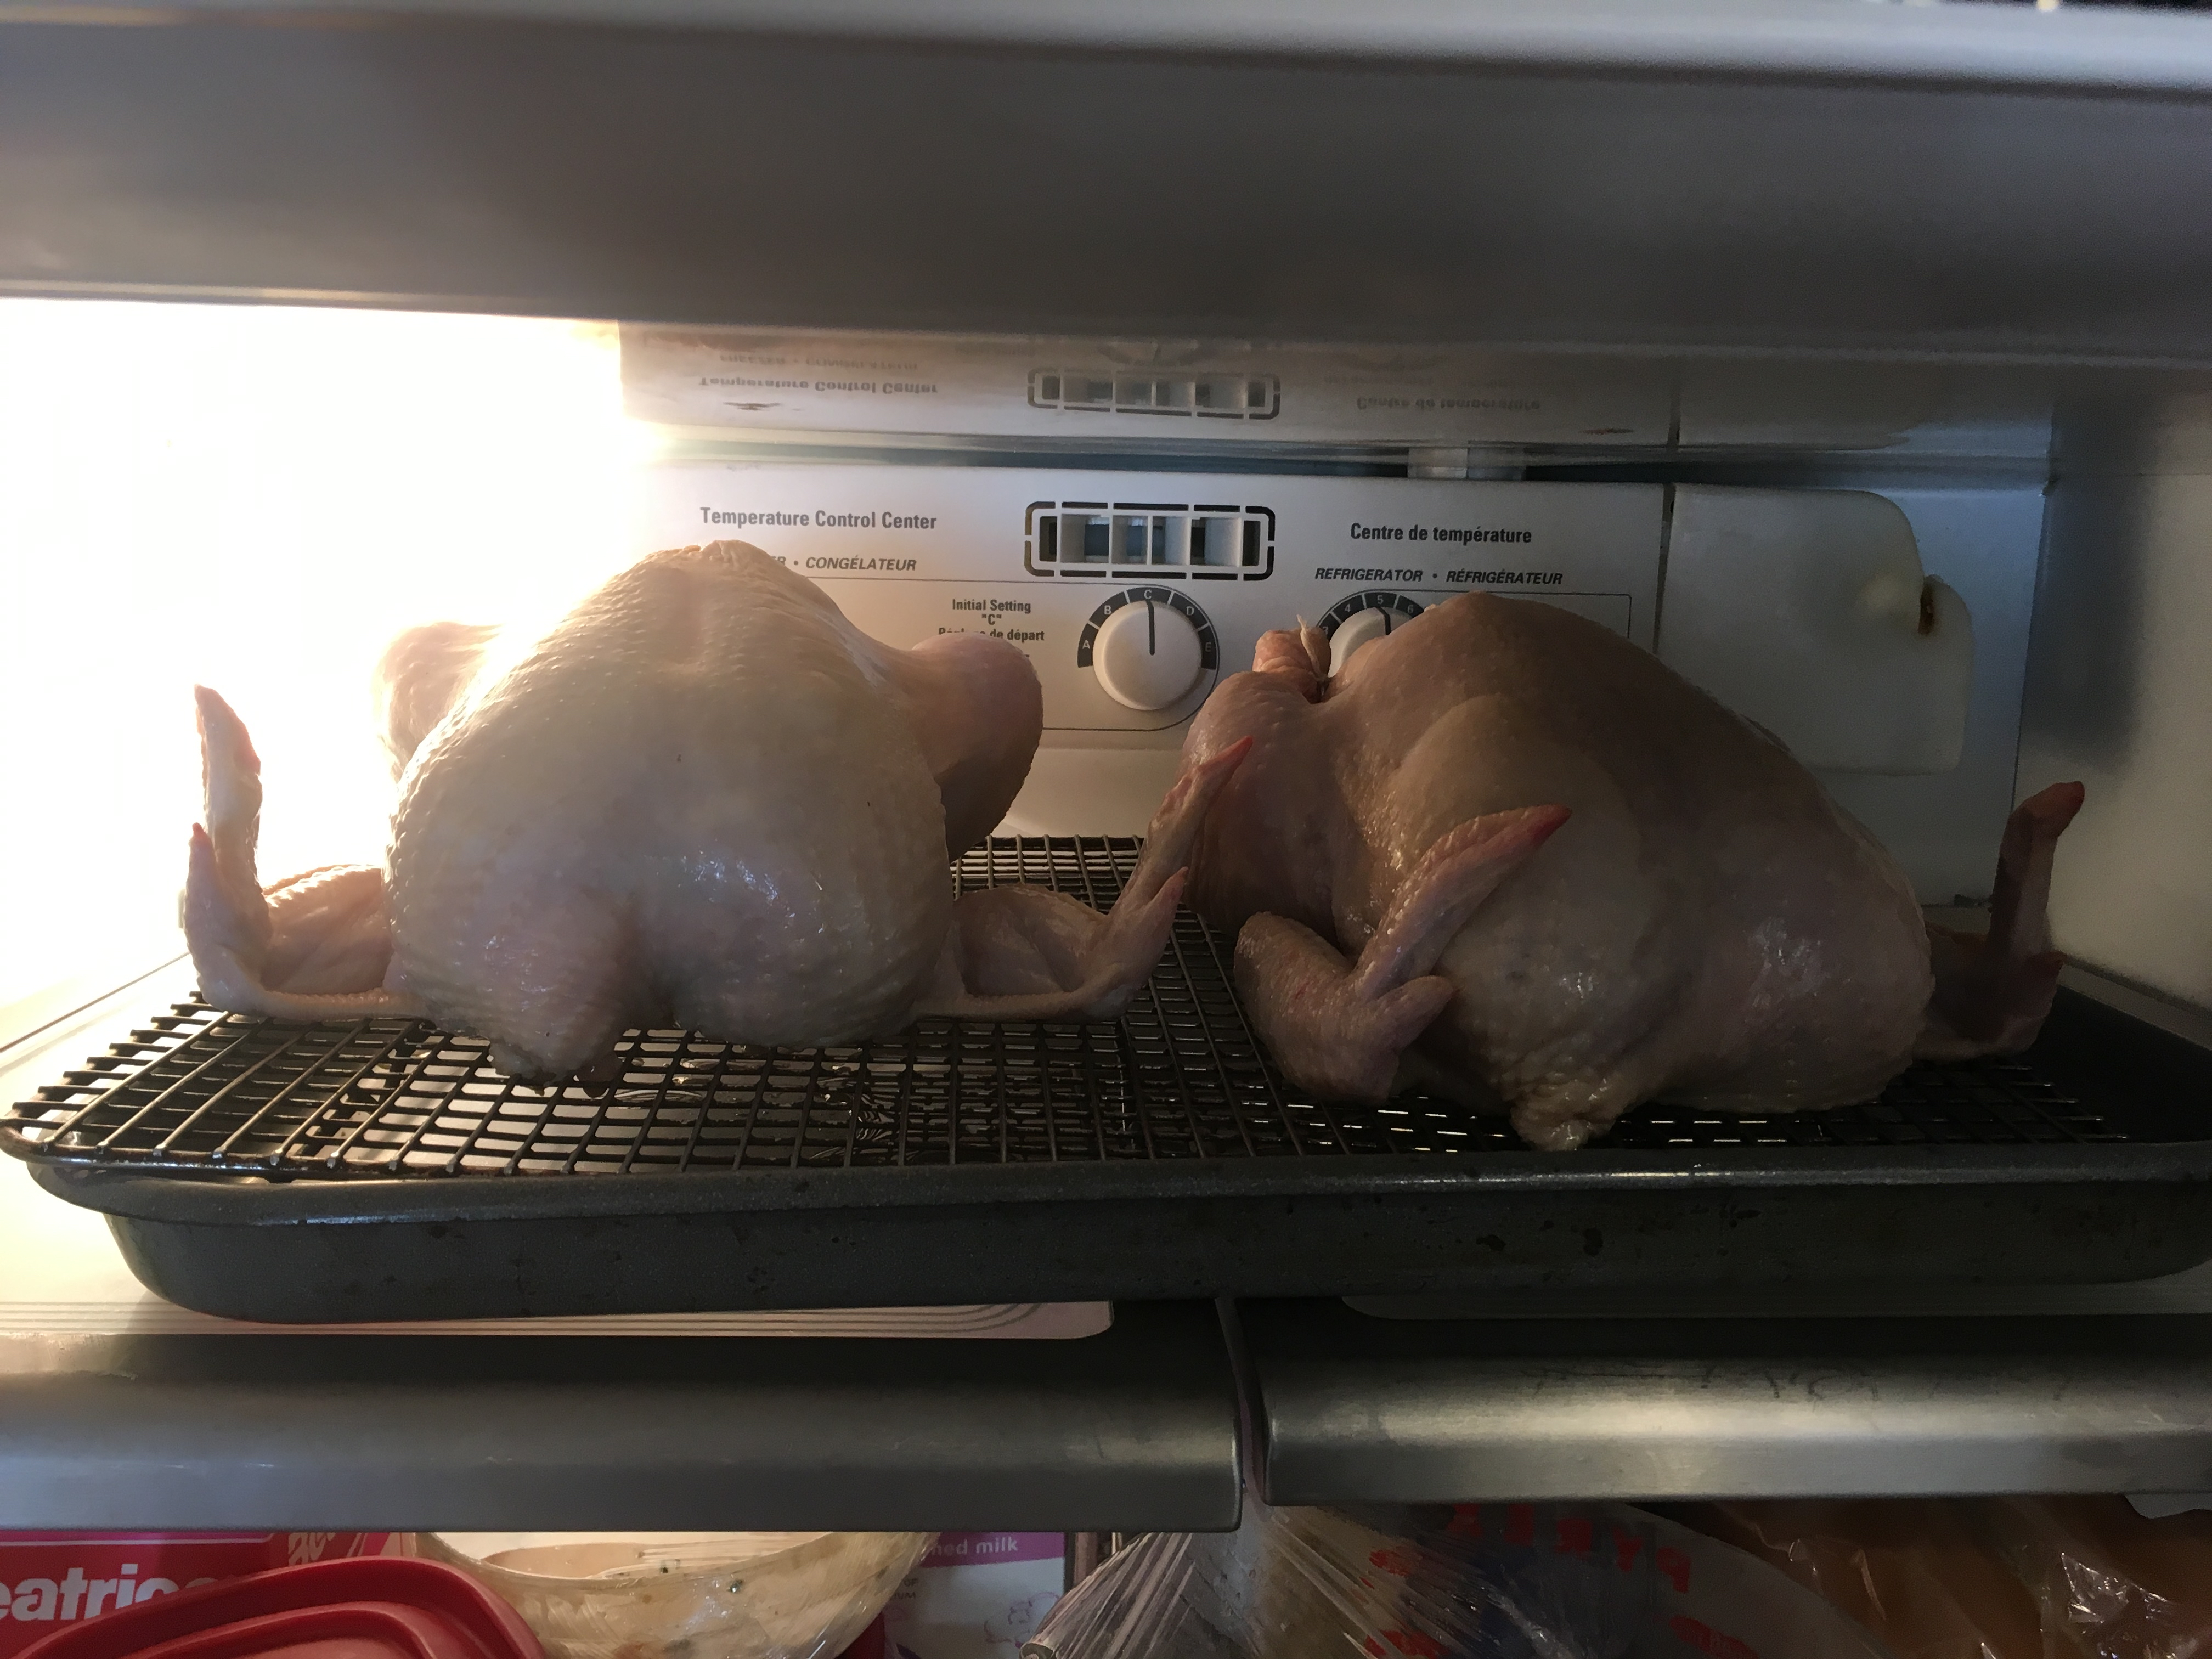
\includegraphics[width=0.25\textwidth]{\imageDir/\fileName/IMG_3220.jpg} &
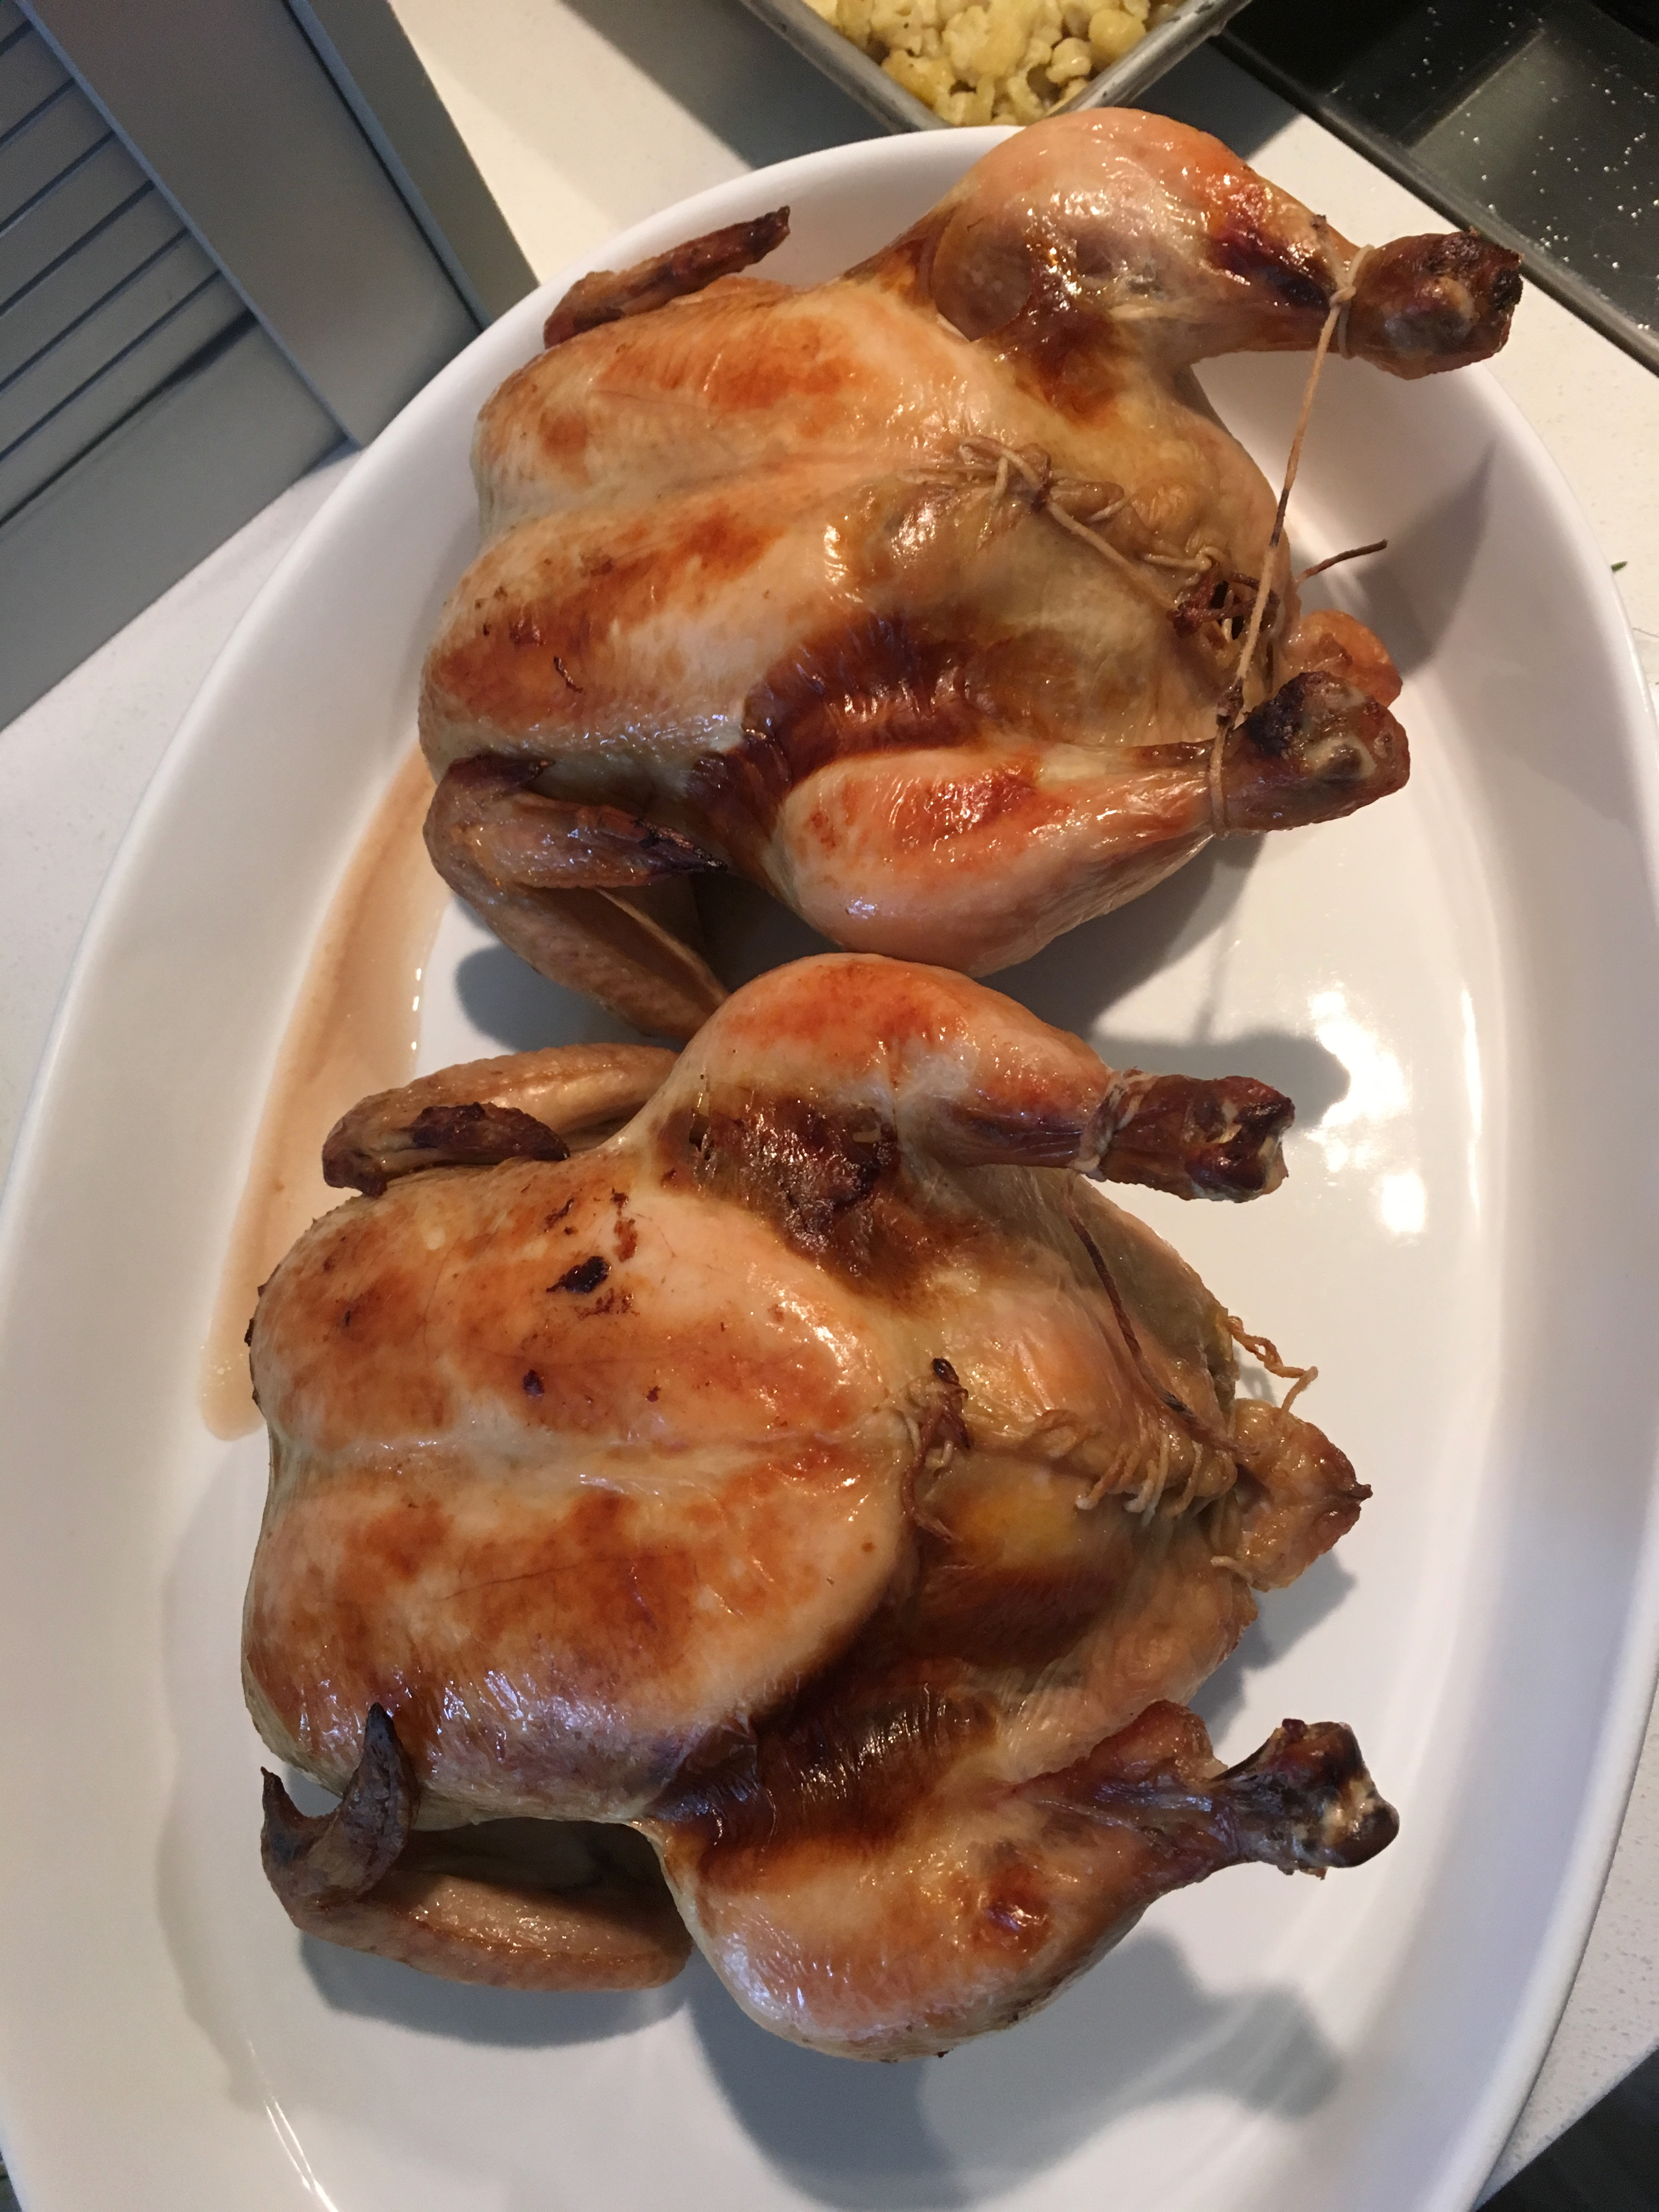
\includegraphics[width=0.25\textwidth]{\imageDir/\fileName/IMG_3228.jpg} \\
\end{tabular}
\end{table}


\end{document}




